\documentclass[12pt,a4paper]{report}
\usepackage[top = 1.6cm, left = 2.7cm, right = 2.7cm ]{geometry}
\usepackage{setspace}
\usepackage[utf8]{inputenc}
\usepackage[francais]{babel}
\usepackage{float}
\usepackage[T1]{fontenc}
\usepackage{amsmath}
\usepackage{amsthm}
\usepackage{amsfonts}
\usepackage{amssymb}
\usepackage{graphicx}
\usepackage{hyperref}
\usepackage{amsthm,thmtools}
\usepackage{cite}
\usepackage{bbm} 
\usepackage{xcolor}
\usepackage{framed}
\colorlet{shadecolor}{lightgray!25}

%% Theorem Styles %%

\theoremstyle{definition}%{3pt}{3pt}{\slshape}{}{\bfseries}{.}{.5em}{}
\newtheorem{definition}{Définition}[chapter]
\newtheorem{theorem}{Théorème}[chapter]
\newtheorem*{notation}{Notation}
\newtheorem{propriete}{Propriété}[chapter]
\newtheorem*{proprietes}{Propriétés}
\newtheorem{proposition}{Proposition}[chapter]
\theoremstyle{remark}
\newtheorem{example}{Exemple}[chapter]
\newtheorem{remark}{Remarque}[chapter]

%%Definition by chapter%%

\usepackage{etoolbox}
\makeatletter
\patchcmd\thmtlo@chaptervspacehack
{\addtocontents{loe}{\protect\addvspace{10\p@}}}
{\addtocontents{loe}{\protect\thmlopatch@endchapter\protect\thmlopatch@chapter{\thechapter}}}
{}{}
\AtEndDocument{\addtocontents{loe}{\protect\thmlopatch@endchapter}}
\long\def\thmlopatch@chapter#1#2\thmlopatch@endchapter{%
	\setbox\z@=\vbox{#2}%
	\ifdim\ht\z@>\z@
	\hbox{\bfseries\chaptername\ #1}\nobreak
	#2
	\addvspace{10\p@}
	\fi
}
\def\thmlopatch@endchapter{}

\makeatother
\renewcommand{\thmtformatoptarg}[1]{ -- #1}

%% Commandes persos %%
\newcommand\bbone{\ensuremath{\mathbbm{1}}}
\newcommand{\eg}{e.g. }
\newcommand{\ssi}{ssi }
\newcommand{\ie}{i.e., }
\newcommand{\cf}{cf. }
\newcommand{\pr}{\mathbb{P}}
\renewcommand{\listtheoremname}{Définitions et théorèmes}

\setstretch{1,1}
\let\labelitemi\labelitemii


\begin{document}
\begin{titlepage}
	
	\newcommand{\HRule}{\rule{\linewidth}{0.5mm}} % Defines a new command for the horizontal lines, change thickness here
	
	\center % Center everything on the page 
	%----------------------------------------------------------------------------------------
	%	HEADING SECTIONS
	%----------------------------------------------------------------------------------------
	

	\begin{center}
	
\includegraphics[height=2cm]{logos/UMONS_FS.pdf}
	\hspace{5cm}
	
\includegraphics[height=1.7cm]{logos/UMONS+txt}
	\\[1em]
	\vspace{1cm}
	\end{center}
	\textsc{\large Service d'informatique théorique }\\[0.5cm] % Major heading such as course name
	
	%\vspace{1cm}
	%----------------------------------------------------------------------------------------
	%	TITLE SECTION
	%----------------------------------------------------------------------------------------
	
	\vspace{0.5cm}
	\HRule \\[0.4cm]
	{ \huge \bfseries Jeux avec plus court chemin}\\[0.4cm] % Title of your document
	\HRule \\[1cm]
	%{\large Projet de Master 1}
	
	%----------------------------------------------------------------------------------------
	%	AUTHOR SECTION//
	%----------------------------------------------------------------------------------------
	\vspace{2cm}
	\begin{minipage}{0.4\textwidth}
		\begin{flushleft} \large
			\emph{Auteur :} \\Florent Delgrange
		\end{flushleft}
	\end{minipage}
	~
	\begin{minipage}{0.4\textwidth}
		\begin{flushright} \large
			\quad \\
			\emph{Directeurs:}\\ \quad Véronique Bruyère \\ \quad Mickaël Randour\\	\vspace*{0.5cm}
			\emph{Rapporteur:}\\
			Quentin Hautem
		\end{flushright}
		
	\end{minipage}\\[5cm]
	
	% If you don't want a supervisor, uncomment the two lines below and remove the section above
	%\Large \emph{Author:}\\
	%John \textsc{Smith}\\[3cm] % Your name
	
	%----------------------------------------------------------------------------------------
	%	DATE SECTION
	%----------------------------------------------------------------------------------------
	\vspace{4cm}
	%{\large \today}\\[3cm] % Date, change the \today to a set date if you want to be precise
	\begin{center}
			Ann\'ee acad\'emique 2016-2017
	\end{center}
	
	%----------------------------------------------------------------------------------------
	%	LOGO SECTION
	%----------------------------------------------------------------------------------------
	
	\vspace*{1cm}

	
	%----------------------------------------------------------------------------------------
	
	\vfill % Fill the rest of the page with whitespace
	
\end{titlepage}

\newpage
\tableofcontents
\listoftheorems[ignoreall,show={definition,theorem}]
\newpage

\chapter*{Introduction}

\chapter{Introduction aux probabilités}
Les processus décisionnels Markovien sont des automates qui modélisent des phénomènes aléatoires enrichis par des probabilités. Avant de définir formellement de tels modèles, il est utile d'introduire brièvement quelques notions de probabilités qui seront indispensables à la compréhension de la suite du document.

\begin{definition}[\textbf{$\sigma$-algèbre}]
	Une $\sigma$-algèbre est une paire $(\Omega, \sigma)$ où $\Omega$ est un ensemble non-vide et $\sigma \subseteq \mathcal{P}(\Omega)$ qui respecte les $3$ conditions suivantes :
	\begin{enumerate}
		\item $\varnothing \in \sigma$
		\item Si $E \in \sigma$, alors $\overline{E} = \Omega \setminus E$ et $\overline{E} \in \sigma$
		\item Si $E_1, E_2, \dots \in \sigma$, alors $\bigcup_{n \geq 1} E_n \in \sigma$
	\end{enumerate}
	Les éléments de $\Omega$ sont appelés \textit{résultats} et les éléments de $\sigma$ sont appelés \textit{évènements}.
\end{definition}

\begin{remark} \label{probaremark}
	Ces conditions sur la $\sigma$-algèbre mènent au fait que
	\begin{itemize}
		\renewcommand{\labelitemi}{\tiny$\bullet$}
		\item
	$\Omega \in \sigma$. En effet, on a que $\Omega$ est non-vide par définition et $\varnothing \in \sigma$. Donc, $\overline{\varnothing} = \Omega \setminus \varnothing = \Omega \in \sigma$.
		\item 	$\sigma$ est fermé par des intersections dénombrables, \ie $\forall E \in \sigma$ et $\forall n$ tel que $E_n \subseteq E$,
		\[ \bigcap_{n \geq 0} E_n = \overline{\bigcup_{n \geq 0} \overline{E_n}}\]
		En effet, $\bigcup_{n \geq 0} \overline{E_n} \text{ avec } \overline{E_n}  = \Omega \setminus E_n \in \sigma$ est \textit{l'union des ensembles formés de tous les éléments de $\Omega$ non-contenus dans chaque ensemble $E_n$}. \\
		$\overline{\bigcup_{n \geq 0} \overline{E_n}} = \Omega \setminus \big(\bigcup_{n \geq 0} \overline{E_n} \big) \in \sigma$ est donc \textit{l'ensemble des éléments contenus dans tous les ensembles $E_n$}, \ie $\bigcap_{n \geq 0} E_n$.
	\end{itemize}
\end{remark}
\begin{remark}[\textit{Cas particuliers}]
		Si $\sigma = \mathcal{P}(\Omega)$, alors tous les sous-ensembles de $\Omega$ sont des évènements. Si
		$\sigma = \{\varnothing, \Omega\}$, alors $\forall E \subset \Omega$ tel que $E \neq \varnothing$, on a que $E \notin \sigma$, \ie tout sous-ensemble non-vide strict de $\Omega$ n'est pas un évènement.
\end{remark}

\begin{definition}[\textbf{Mesure de probabilité}]\label{proba_measure} Soit $(\Omega, \sigma)$, une $\sigma$-algèbre.
	Une mesure de probabilité sur $(\Omega, \sigma)$ est une fonction $\mathbb{P} : \sigma \rightarrow [0, 1]$ telle que
	\begin{itemize}
		\renewcommand{\labelitemi}{\tiny$\bullet$}
		\item $\mathbb{P}(\Omega) = 1$
		\item Si $(E_n)_{n \geq 1}$ est une suite d'évènements disjoints $E_n \in \sigma$, alors:
		\[\mathbb{P}(\bigcup_{n \geq 1} E_n) = \sum_{n \geq 1} \mathbb{P}(E_n)\]
	\end{itemize}
	On dit alors que $(\Omega, \sigma, \mathbb{P})$ est un \textit{espace probabiliste}.
	On appelle $\mathbb{P}(E)$ la mesure de probabilité de l'évènement $E$ ou encore plus simplement la probabilité de $E$.
\end{definition}

\begin{definition}[\textbf{Distribution de probabilité}] \label{distriprobadef}
	Soit $(\Omega, \sigma)$, une $\sigma$-algèbre. 
	On suppose que $\Omega$ est un ensemble dénombrable. Alors, il existe une fonction $\mu: \Omega \rightarrow [0,1]$, une mesure de probabilité telle que 
	\[\sum_{\omega \in \Omega} \mu(\omega) =1 \]
	$\mu$ est appelée \textit{distribution de probabilité sur $\Omega$}. Pour avoir une mesure de probabilité sur la $\sigma$-algèbre dont $\sigma = \mathcal{P}(\Omega)$, il suffit d'avoir $\mu$ sur $\Omega$ et d'étendre $\mu$ à $\pr$ de la façon suivante :
	\[ \forall E \in \sigma,\; \mathbb{P}_{\mu}(E) = \sum_{\omega \in E} \mu(\omega)\] On dit que $P_{\mu}$ est la mesure de probabilité induite par la distribution de probabilité $\mu$.
\end{definition}

\subsection*{Propriétés}
	Nous allons maintenant introduire quelque propriétés que nous allons utiliser au fil du document.
	Soit $(\Omega, \sigma, \mathbb{P})$, un espace probabiliste. 
	
\begin{propriete} \label{negproba}
$\forall E \in \sigma$, $\mathbb{P}(E) = 1 - \mathbb{P}(\overline{E})$. En particulier, $\mathbb{P}(\varnothing) = 0$ (car $\mathbb{P}(\Omega) = 1$).
\end{propriete}
\begin{propriete}[\textit{Les mesures de probabilité sont monotones}]
\[\forall E, E' \in \sigma \text{ tel que } E \subseteq E',\; \mathbb{P}(E') = \mathbb{P}(E) + \mathbb{P}(E' \setminus E) \geq \mathbb{P}(E)\]

	De ce fait, soit $(E_n)_{n \geq 1}$, une suite d'évènements (pas forcément disjoints). \[\bigcup_{n \geq 1} E_n = \bigcup_{n \geq 1} E'_n \text{ où }E_1 = E'_1\text{ et }E'_n = E_n \setminus (E_1 \cup E_2 \cup \dots \cup E_{n-1}) \;\; \forall n \geq 2\]
		Par définition de $(E'_n)_{n \geq 1}$, on a toujours que $E'_n \cap E'_m = \varnothing$ quand $n \neq m$ (tous les éléments de la suite sont des ensembles disjoints), et donc
		\[ \mathbb{P}(\bigcup_{n \geq 1} E_n) =  \mathbb{P}(\bigcup_{n \geq 1} E'_n) = \sum_{n \geq 1}\mathbb{P}(E'_n) \quad \text{\textit{(par la définition \ref{proba_measure})}}\]
		Supposons à présent que $E_1 \subseteq E_2 \subseteq E_3 \subseteq \dots$, alors, on a :
		\begin{flalign}
			\mathbb{P}(\bigcup_{n \geq 1} E_n) 
				&= \pr(E_1) + \sum_{n=2}^\infty (\pr(E_n) - \pr(E_{n-1})) \notag \\
				&= \pr(E'_1) + \sum_{n=2}^\infty \pr(E'_n) \notag \\
				&= \lim_{n \rightarrow \infty} \pr(E_n) \notag
		\end{flalign}
		et $\mathbb{P}(E_1) \leq \mathbb{P}(E_2) \leq \dots \leq \mathbb{P}(E_n) \leq 1$.
\end{propriete}
\begin{propriete}
		Soit $(E_n)_{n \geq 1}$, une suite d'évènements. 
		Supposons que $E_1 \supseteq E_2 \supseteq E_3 \supseteq \dots$, alors :
		\[ \mathbb{P}(\bigcap_{n \geq 1} E_n) = \lim_{n \rightarrow \infty} \mathbb{P}(E_n)\]
		En effet, par le fait que $\forall n, \; E_n \supseteq  {E_{n +1}} \iff \overline{E_n} \subseteq \overline{E_{n +1}}$ (car $\overline{E_n} = \Omega \setminus E_n$),
		\begin{flalign}
			\pr\big(\bigcap_{n \geq 1} E_n \big)
			&= \pr\big(\overline{\bigcup_{n \geq 1} \overline{E_n}}\big) \tag{\textit{par la remarque \ref{probaremark}}} \\
			&= 1 - \pr\big(\bigcup_{n \geq 1} \overline{E_n} \big) \tag{\textit{par la propriété \ref{negproba}}} \\
			&= 1 - \lim_{n \rightarrow \infty} \pr(\overline{E_n}) \tag{\textit{par la monotonicité}} \\
			&= 1 - \lim_{n \rightarrow \infty} \big(1 - \pr(E_n)\big) \notag\\
			&= \lim_{n \rightarrow \infty} \mathbb{P}(E_n) \notag
		\end{flalign}
\end{propriete}

\begin{example}[\textit{Lancer d'un dé}]\label{die}
	On lance un dé. Chaque face a exactement une chance sur six d'apparaitre suite à ce lancer de dé. On définitformellement le $\sigma$-algèbre correspondant à ce lancer de dé : 
	Les résultats sont $\Omega = \{1, 2, 3, 4, 5, 6\}$ et les évènements sont $\sigma = \mathcal{P}(\Omega)$.
	On sait qu'il existe une fonction $\mu: \Omega \rightarrow [0,1]$ telle que $\mu$ est une distribution de probabilité. Prenons $\mu(\omega) = \frac{1}{6} \; \text{ pour tout } \omega \in \Omega$.\\
	On est à présent intéressé par la probabilité des évènements suivants à l'aide de la mesure de probabilité $\pr_{\mu}$ induite par $\mu$:
	\begin{itemize}
		\renewcommand{\labelitemi}{\tiny$\bullet$}
		\item "Le résultat du lancer de dé est 1 ou 6" = $\{1, 6\} \in \sigma$
		\[\pr_{\mu}(\{1,6\}) = \mu(1) + \mu(6) = \frac{1}{6} + \frac{1}{6} = \frac{1}{3}\]
		\item "Le résultat du lancer de dé n'est pas 1 ou 6" = $\overline{\{1, 6\}} = \{2, 3, 4, 5\}$
		\[\pr_{\mu}(\{2, 3, 4, 5\}) = 1 - \pr_{\mu}(\{1, 6\}) = 1 - \frac{1}{3} = \frac{2}{3}\]
	\end{itemize}
\end{example}

\subsection*{Espérance mathématique}
Nous serons par la suite, à de nombreuses reprises, confrontés à la notion d'\textit{espérance}. Il est donc intéressant d'introduire les concepts liés à cette notion.

\begin{definition}[\textbf{Variable aléatoire}]~\cite{Course2} \\
	Soient $I \subseteq \mathbb{N}, \; \mathcal X = (x_i)_{i \in I}$, un ensemble dénombrable et $(\Omega, \sigma, \pr)$, un espace probabiliste. Soit $X$, une application telle que
	\[X :
	\begin{cases}
	(\Omega, \sigma, \pr) \rightarrow \mathcal{X} = (x_i)_{i \in I} \\
	\omega \mapsto X(\omega)
	\end{cases}
	\]
	est une \textit{variable aléatoire} si 
	\[\forall i \in I, \quad \{X = x_i\} = \{\omega \in \Omega \; | \; X(\omega) = x_i \} \in \sigma\]
	\ie si on peut faire correspondre chaque élément de $\mathcal{X}$  à un évènement de l'espace probabiliste. Cette condition assure que tout ensemble $\{X = x_i\}$ possède une probabilité mesurable par $\pr$.
\end{definition}

\begin{example}[\textit{Parité lors d'un lancer de dé}]
	On lance un dé (\cf exemple \ref{die}) et on est intéressé de savoir si la face du dé qui apparait est paire ou impaire. On définit la variable aléatoire discrète $X:(\Omega, \sigma, \pr_{\mu}) \rightarrow \mathcal{X} = \{pair, impair\}$. On a $\{X = pair\} = \{2, 4, 6\}$ et $\{X = impair\} = \{1, 3, 5\}$. Dès lors $\pr_{\mu}(X = pair) = \pr_{\mu}(\{2, 4, 6\}) =\frac{1}{2} = \pr_{\mu}(X = impair) = \pr_{\mu}(\{1, 3, 5\})$.
\end{example}

\begin{definition}[\textbf{Espérance}]\label{espmath}\cite{Course2}\\
	Soit $X$, une variable aléatoire réelle. On définit $\mathbb{E}[X]$ comme étant \textit{l'espérance} de $X$ où 
	\[\mathbb{E}[X] = \sum_{i \in I}x_i \cdot \pr(X = x_i) \]
	\ie l'espérance de $X$ est \textbf{la moyenne pondérée} des valeurs $x_i$ par la probabilité que $X = x_i$ ou encore la moyenne de $X$.
	
\end{definition}
\begin{example}[\textit{Espérance d'un lancer de dé}]
	On suppose qu'on lance un dé (\cf exemple \ref{die}). Soit $X$, une variable aléatoire représentant les faces du dé. On a 
	\[ \mathbb{E}[X] = \sum_{x = 1}^6 x \cdot \pr(X = x)  = \frac{1}{6} \sum_{x = 1}^6 x = \frac{1}{6} \cdot \frac{6 \cdot 7}{2} = \frac{7}{2}\] \ie l'espérance d'un lancer de dé est $3.5$.
\end{example}

%\begin{example}[\textit{Lancers d'une pièce}]
%	On lance une infinité de fois une pièce. Le résultat d'un lancer de pièce est soit pile, soit face et la chance que le résultat de ce lancer de pièce soit pile est la même que le résultat soit face. L'ensemble des résultats $\Omega$ d'un lancer infini d'une pièce est donc l'ensemble des suites formées de pile ou de face, \ie, $\omega = \{x_1, x_2, \dots\} \in \Omega$ avec $x_n \in \{pile,\; face\} \;\; \forall n \in \mathbb{N}_0$. Cette fois, $\Omega$ est infini mais est toujours dénombrable. 
%\end{example}

\chapter{Chaînes de Markov}

Insérer ici une introduction aux chaînes de Markov et une définition non-formelle.\\

Les définitions proposées dans ce document sont inspirées du chapitre \textit{Probabilistic Systems} du livre \textit{Principles of model checking} ~\cite{DBLP:books/daglib/0020348} ainsi que du chapitre intitulé \textit{Model Checking Probabilistic Systems} du cours de Mickaël Randour (\textit{Formal verification of computer systems}) ~\cite{Course1}.

\section{Définitions et propriétés}

\theoremstyle{definition}
\begin{definition}[\textbf{Chaîne de Markov à temps discret}]
	
	Une \textit{chaîne de Markov à temps discret}, notée \textbf{CM}, est un automate probabiliste défini par un tuple  $\mathcal{M} = (S, \Delta)$ où :
	\begin{itemize}
		\renewcommand{\labelitemi}{\tiny$\bullet$}
		\item $S$ est un ensemble dénombrable d'états.
		\item $\Delta: S \times S \rightarrow [0,1] \cap \mathbb{Q}$ est la \textit{fonction de transition} telle que \[\forall s \in S, \sum_{s' \in S}\Delta(s, s')= 1\]
		%\item $d_0:S \rightarrow [0,1]$ est la distribution initiale telle que \[\sum_{s \in S}d_0(s)= 1\] (à noter que dans le cadre de ce document, la distribution initiale peut être omise, et dans ce cas, $\forall s \in S, d_0(s) = \frac{1}{|S|}$).
		$\Delta$ spécifie, pour tout état $s \in S$, la probabilité de passer de l'état $s$ à l'état $s'$. 
	\end{itemize}
	On dit que $\mathcal{M}$ est \textit{finie} si $S$ est un ensemble fini.
\end{definition}

\begin{propriete} \label{distribmarkov}
	Soient $\mathcal{M} = (S, \Delta)$ et $s \in S$.
	Les contraintes imposées sur $\Delta$ assurent que $\Delta(s, \cdot)$ est une distribution de probabilité sur $S$  (par la définition \ref{distriprobadef}) avec \[\Delta(s, \cdot) : S \rightarrow [0, 1] \cap \mathbb{Q}, \; s' \mapsto \Delta(s, s')\] On dénote par $\pr_s$ la mesure de probabilité induite par la distribution de probabilité $\Delta(s, \cdot)$.%$ \Delta(s, s') \; \forall s'$.
\end{propriete}
%Plus strictement, soit $X_n$, une variable aléatoire représentant l'état du système après $n \in \mathbb{N}$ étapes, \[\Delta(s, s') = \mathbb{P}(X_{n+1} = s' | X_n = s) \]
%$\Delta(s, s')$ est donc la probabilité que le système se trouve en l'état $s'$ à l'étape $n+1$ alors qu'il se trouvait en l'état $s$ à l'étape $n$. \\
%La valeur $d_0(s)$ spécifie la probabilité de commencer dans le système en l'état $s$. Si $d_0(s) > 0$, alors $s$ est appelé \textit{état initial}.% De la même manière, $d_0(s) = \mathbb{P}(X_0 = s)$.

\begin{definition}[\textbf{Graphe sous-jacent d'une chaîne de Markov}]
	Une CM $\mathcal{M} = (S, \Delta)$ induit un \textit{graphe sous-jacent} (orienté) $G^\mathcal{M} = (V, E)$ où :
	\begin{itemize}
		\renewcommand{\labelitemi}{\tiny$\bullet$}
		\item $V$ est l'ensemble de sommets du graphe tel que $|V| = |S|$, \ie il existe une bijection de $S$ vers $V$. Chaque sommet $s' \in V$ est donc associé à un unique état $s \in S$. Par abus de langage, on dit que $V = S$.
		\item $E$ est l'ensemble des arcs du graphe tel que \[ \forall s, s' \in S, \; (s, s') \in E \text{ \ssi} \Delta(s, s') > 0\]
	\end{itemize}
\end{definition}

Afin d'illustrer une chaîne de Markov, on utilise la représentation de son graphe sous-jacent où 
%\begin{itemize}
%	\renewcommand{\labelitemi}{\tiny$\bullet$}
%	 \item
chaque arc $(s, s') \in E$ est étiqueté par la probabilité de passer de l'état $s$ à l'état $s'$ en une étape : $\Delta(s, s')$.
	 %\item Si $\exists s, s' \in S$ tel que $d_0(s) \neq d_0(s')$, alors chaque état initial $s$ est illustré par un arc allant du vide vers le sommet $s$.
%\end{itemize}

\begin{example} [\textit{Simuler un lancer de dé avec une pièce de monnaie}] \label{knuthdie}
	On génère le comportement d'un dé via une pièce de monnaie selon l'algorithme probabiliste de Knuth et Yao ~\cite{KY76}. Cet algorithme est simulé à l'aide de la chaîne de Markov $\mathcal{M}_{Kd}$ illustrée à la figure ~\ref{diebyacoin}.
	\begin{figure}[H]
		\centering
		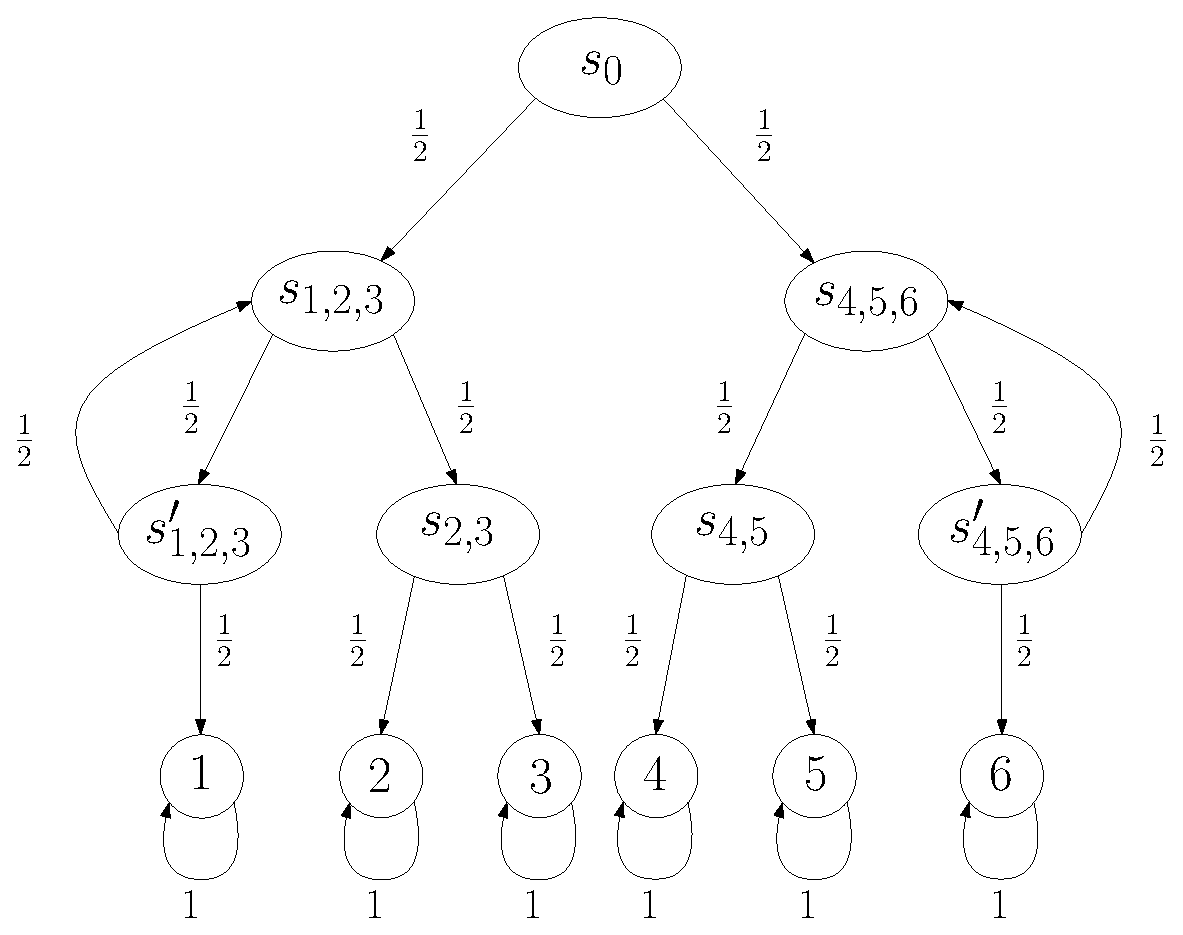
\includegraphics[scale=0.5]{figures/dieByaCoin.eps}
		\caption{Simulation d'un lancer de dé avec une pièce par une chaîne de Markov}
		\label{diebyacoin}
	\end{figure}
	On commence en l'état $s_0$, qu'on appellera ici l'état initial. Les états $1, 2, 3, 4, 5, 6$ sont appelés états finaux et représentent les différentes faces du dé (\ie les résultats possibles du lancer de dé), tandis que les états internes ($\notin \{s_0, 1, 2, 3, 4, 5, 6\}$) représentent les états du système après un lancer de pièce.
	 Pour tout état interne, un lancer de pièce dont le résultat est face emprunte l'arc de gauche pour déterminer son état suivant. Un lancer de pièce dont le résultat est pile emprunte l'arc de droite pour déterminer son état suivant. Lorsqu'on lance un dé, la probabilité de tomber sur n'importe quelle face du dé est exactement de $\frac{1}{6}$. Le comportement du modèle doit donc simuler ce phénomène lorsqu'un état final est atteint.\\
	
	\textit{Simulation : }On suppose que le système démarre en l'état $s_0$. On lance une pièce. Si le résultat est face, le système évolue en l'état $s_{1, 2, 3}$. La probabilité que le résultat du lancer de pièce soit pile est égale à la probabilité que le résultat du lancer de pièce soit face. Par conséquent, en relançant la pièce, la probabilité que le système évolue en $s_{2, 3}$ est égale à la probabilité que le système évolue en $s'_{1, 2, 3}$. Si le système évolue en $s'_{1, 2, 3}$, un lancer de pièce mène à la face 1 du dé avec une probabilité $\frac{1}{2}$, égale à la probabilité de retourner en l'état $s_{1, 2, 3}$. Sinon, le système évolue en $s_{2, 3}$ et un lancer de pièce mènera obligatoirement au résultat d'un lancer de dé (avec une probabilité $\frac{1}{2} \text{ ou avec une probabilité }  \frac{1}{2}$, et donc avec une probabilité $1$), à savoir la face 2 ou 3. Le comportement du système se trouvant dans l'état $s_0$ dans le cas où le résultat du lancer de pièce est pile est symétrique.\\
	
	On verra plus tard dans ce document qu'en simulant un lancer de dé par une pièce, en suivant le système décrit par la CM $\mathcal{M}_{Kd}$ et en démarrant en l'état $s_0$, chaque face du dé est atteint avec une probabilité $\frac{1}{6}$.\\
	
\end{example}

\begin{definition}[\textbf{Matrice de transition}]
	Soient $\mathcal{M} = (S, \Delta)$, une CM et $n = |S|$. On suppose que $S$ est dénombrable. On peut dès lors énumérer les états de $S$. Soient $i,j \in \{1, \dots, n\}$ ($s_i \in S$, est le $i^{\text{ème}}$ sommet de $S$ et $s_j \in S$ est le $j^{\text{ème}}$ sommet de $S$). Soit \textbf{P}$\in \mathbb{Q}^{n \times n}$. On dit que
	\textbf{P} est \textit{la matrice de transition} de $\mathcal{M}$ \ssi $\textbf{P}_{i,j} = \Delta(s_i, s_j)$.\\
			 %\item $a^{(0)} \in \mathbb{R}^n$ est le vecteur initial de $\mathcal{M}$ \ssi $a^{(0)}_i = d_0(s_i)$
			%\end{itemize}
	La ligne $\textbf{P}_{i \cdot}$ contient la probabilité des transitions de l'état $s_i$ vers ses successeurs, tandis que la colonne $\textbf{P}_{\cdot j}$ spécifie la probabilité, pour tout état $s$, d'atteindre l'état $s_j$ en une étape.
\end{definition}

\begin{example}[\textit{Modèle d'Ehrenfest pour la diffusion des gaz ~\cite{Course3}}]
	Le modèle est proposé par Ehrenfest pour décrire les échanges de chaleur entre deux systèmes portés initialement à une température différente. On modélise la répartition de $N$ molécules de gaz à l'intérieur d'un récipient divisé en deux compartiments (urnes) séparés par une membrane poreuse.\\
	Pour cet exemple simplifié, on prend $N = 4$. Les 2 urnes contiennent $4$ molécules à tout moment et, à chaque étape, une des $4$ molécules est choisie au hasard et change d'urne (\cf figure ~\ref{ehrenfestscheme}).
	\begin{figure}[H]
		\centering
		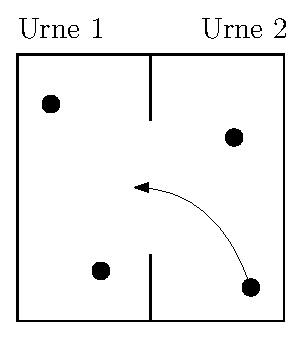
\includegraphics[scale=0.5]{figures/EhrenfestUrne.eps}
		\caption{Schéma simplifié du principe d'Ehrenfest pour $N=4$ molécules.}
		\label{ehrenfestscheme}
	\end{figure}
	
	On modélise ce phénomène par une chaîne de Markov (\cf figure ~\ref{ehrenfestCM}). Ici, $S=\{(2|2), (1|3), (0|4), (3|1), (4|0) \}$. Soit $s \in S$. Chaque état représente le nombre de molécules présentes dans chacune des urnes. \`A chaque étape, chacune des molécules a exactement $1$ chance sur $4$ de changer d'urne.
	%tel que $s \neq (2|2)$, $d_0(s) = 0$, donc $(2|2)$ est l'unique état initial.

	\begin{figure}[H]
		\centering
		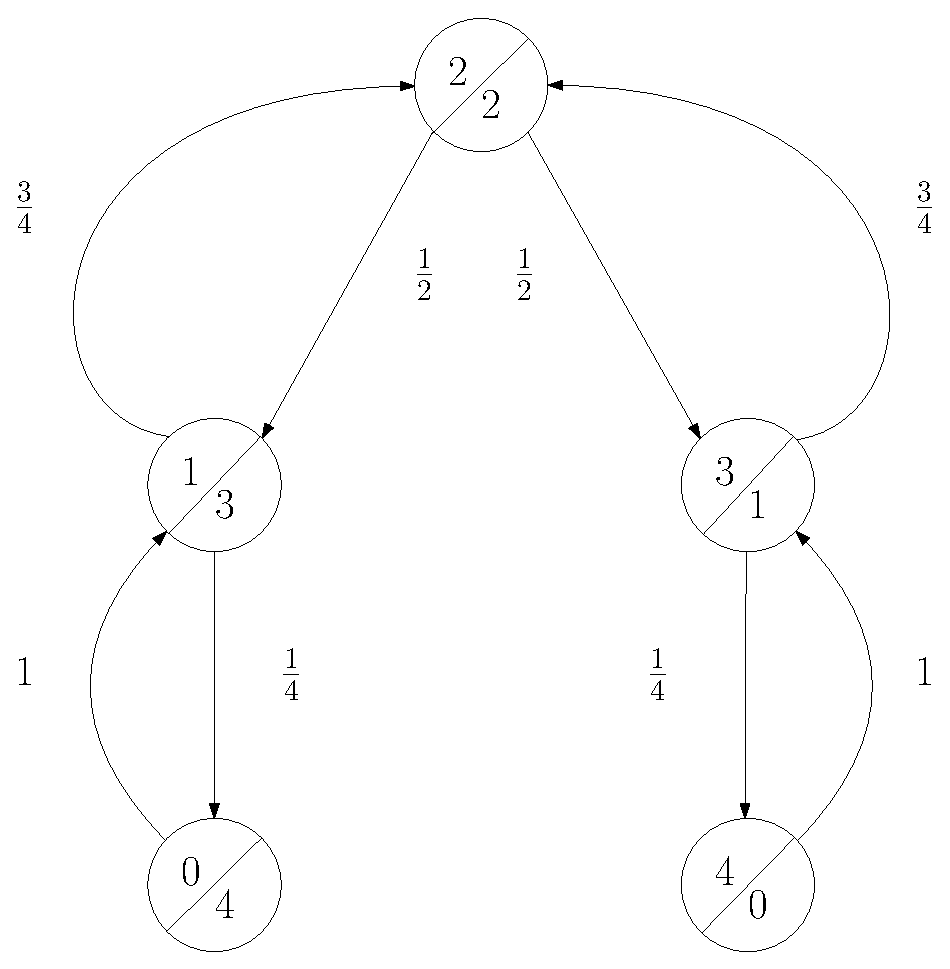
\includegraphics[scale=0.4]{figures/Ehrenfest.eps}
		\caption{Chaine de Markov associée pour $N=4$ molécules}
		\label{ehrenfestCM}
	\end{figure}
	Chaque état de $S$ correspond à la répartition des molécules dans les 2 urnes. Supposons que le système se situe en l'état $(2 | 2)$. On a donc $2$ molécules dans la première ainsi que dans la seconde urne. Alors, par le fait que chaque molécule change d'urne avec une probabilité $\frac{1}{4}$, le système a une probabilité $\frac{1}{4} + \frac{1}{4} = \frac{1}{2}$ d'évoluer en l'état $(1 | 3)$ ou en l'état $(3 | 1 )$. On peut appliquer ce principe pour chaque état. En effet, supposons que le système évolue en $(1 | 3)$. Cela signifie qu'il n'y a qu'une seule molécule dans la première urne, tandis qu'il y a 3 molécules dans la seconde. Par le même principe qu'à l'étape précédente, le système a donc une probabilité $\frac{1}{4}$ d'évoluer en l'état $(0 | 4)$ et une probabilité $\frac{3}{4}$ d'évoluer en l'état $(2 | 2)$.
	\\
	
	En énumérant les état de $S$ comme suit : $(0|4), (1|3), (2|2), (3|1), (4|0)$, on a la matrice $5\times5$ de transition $\textbf{P}$:
	%et le vecteur initial $a^{(0)}$ 
	\[
		\textbf{P} =
			\begin{pmatrix}
			0 & 1 & 0 & 0 & 0 \\
			\frac{1}{4} & 0 & \frac{3}{4}& 0 & 0 \\
			0 & \frac{1}{2} & 0 & \frac{1}{2} & 0 \\
			0 & 0 & \frac{3}{4} & 0 & \frac{1}{4} \\
			0 & 0 & 0 & 1 & 0
			\end{pmatrix}
%			\\, \quad
%		a^{(0)} =
%			\begin{pmatrix}
%			0 \\ 0 \\ 1 \\ 0 \\ 0
%			\end{pmatrix}
	\]
\end{example}

\subsection*{Chemins dans une chaîne de Markov}
On va maintenant s'intéresser aux chemins dans une chaîne de Markov ainsi qu'aux propriétés qui s'y rapportent afin de pouvoir par la suite définir formellement des évènements et calculer leur probabilité dans le but d'être capable de résoudre différents problèmes comme par exemple, celui de \textit{l'accessibilité}.

\begin{definition}[\textbf{Chemin}]
	Soit $\mathcal{M} = (S, \Delta)$, une CM. 
	%On définit un \textit{chemin fini} $\hat{\pi}$ de $\mathcal{M}$ comme étant une séquence d'états $\hat{\pi} = s_0 s_1 s_2 \dots s_n$ tel que $\forall i \in \{0, \dots, n-1\}, s_i \in S$ et $\Delta(s_i, s_{i+1}) > 0$ (en d'autres termes, si l'arc $(s_i, s_{i+1}) \in E$ dans le graphe sous-jacent $G^\mathcal{M} = (S, E)$).
	On définit $\textit{Paths}(\mathcal{M})$ comme étant l'ensemble des \textit{chemins infinis} de $\mathcal{M}$, \ie des séquences $\pi = s_0 s_1 s_2 \dots \in S^\omega$ tel que $\Delta(s_i, s_{i+1}) > 0$ pour tout $i \geq 0$ (en d'autres termes, tel que l'arc $(s_i, s_{i+1}) \in E$ dans le graphe sous-jacent $G^\mathcal{M} = (S, E)$).\\
	De la même façon, on définit $\textit{Paths}_\textit{fin}(\mathcal{M})$, comme étant l'ensemble des chemins finis de $\mathcal{M}$, \ie des séquences $\hat{\pi} = s_0 s_1 s_2 \dots s_n$ tel que $\forall i \in \{0, \dots, n-1\}, s_i \in S$ et $\Delta(s_i, s_{i+1}) > 0$ .\\
	On dénote par $\textit{Paths}(s)$ l'ensemble des chemins infinis qui commencent en l'état $s \in S$ et $\textit{Paths}_\textit{fin}(s)$, l'ensemble des chemins finis qui commencent en l'état $s \in S$.
\end{definition}

\begin{definition}[\textbf{Probabilité d'un chemin}]
	Soient $\mathcal{M}=(S, \Delta)$, une CM, $s \in S$, un état et $\pi = s_0 s_1 \dots \in Paths(s)$, un chemin de $\mathcal{M}$. On suppose que l'état actuel du système est en $s$.
	On défini la mesure de probabilité $\pr_{s}$ sur le $\sigma$-algèbre $(\Omega, \sigma)$ où $\Omega = Paths(s)$ et $\sigma = \mathcal{P}(Paths(s))$ comme étant la probabilité que le système emprunte le chemin $\pi$, ou encore \textit{la probabilité du chemin $\pi$}. Celle-ci est donnée par : 
	\[ \pr_{s}(\{\pi\}) = \Delta(\pi) = \Delta(s_0 s_1 \dots) = \prod_{i \in \mathbb{N}} \Delta(s_i, s_{i+1}) \]
	%\textit{Note : } La probabilité d'un chemin fini $\hat{\pi} = s_0 s_1 \dots s_n$ se définit de la même manière, avec $i \leq n - 1$..
\end{definition}

\begin{propriete} Soient $\mathcal{M} = (S, \Delta)$, une CM et $s \in S$, un état de $\mathcal{M}$.
	La mesure de probabilité $\pr_{s}$ sur $Paths(s)$ est induite par
	\[\Delta_s : Paths(s) \rightarrow [0, 1] \cap \mathbb{Q} \; : \; \pi = s_0 s_1 \dots \mapsto \prod_{i \in \mathbb{N}} \Delta(s_i, s_{i+1}) \]
\end{propriete}

%\begin{proof}
%	On va prouver que $\Delta_s$ est une distribution de probabilité sur $Paths(s)$, c'est à dire .
%\end{proof}

\begin{example}[\textit{Chemins dans le système du dé de Knuth}]
	Pour cet exemple, on reprend la CM de l'exemple \ref{knuthdie}. Soit le chemin $\pi = s_0 s_{1,2,3} s'_{1, 2, 3} s_{1,2,3} s_{2,3} 2^\omega \in Paths(\mathcal{M}_{Kd})$.
	On suppose que l'état actuel du système est $s_0$. Alors, la probabilité que le système emprunte le chemin $\pi$ est $\Delta(\pi) = \Delta(s_0 s_{1,2,3} s'_{1, 2, 3} s_{1,2,3} s_{2,3} 2^\omega) = \frac{1}{2} \cdot \frac{1}{2} \cdot \frac{1}{2} \cdot \frac{1}{2} \cdot \frac{1}{2} \cdot 1 = \frac{1}{2^5} = \frac{1}{32}$
\end{example}

\begin{definition}[\textbf{Préfixe d'un chemin}]
	Soient $\mathcal{M} = (S, \Delta)$, une CM, $s' \in S$, un état de $S$ et $\pi \in Paths(s')$, un chemin de $\mathcal{M}$ commençant en $s'$. On définit $pref(\pi)$ comme étant \textit{l'ensemble des préfixes de $\pi$}, \ie 
	\[ pref(\pi) = \{ \hat{\pi} \in Paths_{fin}(\mathcal{M}) \; | \; \hat{\pi} = s_0 \dots s_n \text{ et } s_n = s' \} \]
	\ie, \textit{l'ensemble des chemins finis de $\mathcal{M}$ se terminant en $s'$}
\end{definition}

\begin{definition}[\textbf{Cylindre d'un chemin fini}]
	Soient $\mathcal{M} = (S, \Delta)$, une CM et $\hat{\pi} \in Paths_{fin}(\mathcal{M})$, un chemin fini de $\mathcal{M}$.  \textit{L'ensemble cylindre} de $\hat{\pi}$ est définit comme suit : 
	\[ Cyl(\hat{\pi}) = \{\pi \in Paths(\mathcal{M}) \; | \; \hat{\pi} \in pref(\pi) \}\]
\end{definition}

\begin{example}[\textit{Cylindre dans le système de dés de Knuth}]
	Reprenons la CM $\mathcal{M}_{Kd}$ définie dans l'exemple \ref{knuthdie}. Soit $\hat{\pi} = s_0s_{1, 2, 3}s_{2, 3} \in Paths_{fin}(\mathcal{M}_{Kd})$. Alors, \[Cyl(\hat{\pi}) = \{ \pi \in Paths(s_{2,3}) \; | \; \pi = s_{2, 3} 2^\omega \text{ ou } \pi = s_{2, 3} 3^\omega \} \]
\end{example}

\begin{propriete}[\textit{Mesure de probabilité du cylindre d'un chemin fini}]
	Soient $\mathcal{M} = (S, \Delta)$, une CM, $s \in S$ et $\hat{\pi} \in Paths_{fin}(s)$, un chemin fini de $\mathcal{M}$. Supposons que le système est actuellement en l'état $s$. Il existe une unique mesure de probabilité $\pr_s$ du cylindre de $\hat{\pi}$ sur $Paths(s)$ et celle-ci est définie par :
	\[\pr_{s}(Cyl(\hat{\pi})) = \Delta(\hat{\pi})\]
	\textit{Intuition} : $\forall s \in S, \; \sum_{\pi \in Paths(s)} \Delta(\pi) = 1 \textit{ car  } \sum_{s' \in S} \Delta(s, s') = 1 $. De ce fait, \[\Delta(s_0 \dots s_n) \cdot \sum_{\pi \in Paths(s_n)} \Delta(\pi) = \Delta(s_0 \dots s_n)\]
\end{propriete}

\section{Problème d'accessibilité}

L'un des problèmes les plus élémentaires de l'étude des chaînes de Markov est de déterminer la probabilité d'atteindre un sous ensemble $T$ d'états cibles du système. La résolution de ce problème est fortement liée à l'étude des problèmes que nous allons rencontrer par la suite dans ce document.

\subsection{\'Enoncé du problème}
Soient $\mathcal{M} = (S, \Delta)$ une CM et $T \subseteq S$, un ensemble d'états cibles. On dénote par $\Diamond T$ l'évènement "\textit{atteindre au moins un état de $T$ via un chemin dans $\mathcal{M}$}". \\
Tout d'abord, il faut s'assurer que la probabilité de $\Diamond T$ est mesurable.
\begin{notation} $Paths_{fin}^T(\mathcal{M})$ désigne l'ensemble des chemins finis dans $\mathcal{M}$ (et $Paths_{fin}^T(s)$ ceux qui commencent en l'état $s \in S$) de la forme $\hat{\pi} = s_0 \dots s_n$ où $s_i \notin T \text{ pour tout } i \in \{0, \dots, n-1\}$ et $s_n \in T$.
\end{notation}
On peut exprimer $\Diamond T$ comme étant l'union dénombrable de tous les cylindres de $\hat{\pi} \in Paths_{fin}^T(\mathcal{M})$. Formellement, $\Diamond T$ est défini de la façon suivante : 
\[
	\Diamond T = \bigcup_{s_0 \dots s_n \in Paths_{fin}^T(\mathcal{M})} Cyl(s_0 \dots s_n)
\]
\begin{notation}
	On dit que \textit{$\pi$ satisfait $\Diamond T$}, \ie $\pi \models \Diamond T$ \ssi $\exists \hat{\pi} = s_0 \dots s_n \in Path_{fin}^T(\mathcal{M}), \; \exists t \in T$ tels que $\exists \pi' \in Paths(t)$, $s_n = t$, $\pi' \in Cyl(\hat{\pi}) $ et $\pi = \hat{\pi} \cdot \pi'$.
\end{notation}
On sait que si le système est actuellement en l'état $s$, une unique mesure de probabilité $\pr_s$ existe sur $Paths(s)$ pour l'ensemble de ces cylindres. Dès lors, étant donné que tous les cylindres sont des ensembles disjoints, soit $s \in S$,
\begin{flalign}
	\mathbb{P}_s (\Diamond T)
	&= \mathbb{P}_s(\{\pi \in \textit{Paths}(s) \; | \; \pi \models \Diamond T\}) \notag \\
	&= \pr_s\big(\bigcup_{s_0 \dots s_n \in Paths_{fin}^T(s)} Cyl(s_0 \dots s_n)\big) \notag \\
	&= \sum_{s_0 \dots s_n \in Paths_{fin}^T(s)} \pr_s(Cyl(s_0 \dots s_n)) \notag \\
	&= \sum_{s_0 \dots s_n \in Paths_{fin}^T(s)} \Delta(s_0 \dots s_n) \notag 
\end{flalign}

est la probabilité qu'un chemin commençant en l'état $s$ satisfasse l'évènement $\Diamond T$, ou encore la probabilité d'atteindre un état de $T$ depuis l'état $s$ via un chemin dans $\mathcal{M}$.\\
On définit $x_s = \mathbb{P}_s(\Diamond T)$ pour tout $s \in S$. On obtient de cette façon un système d'équations linéaire. De ce fait, résoudre $x_s$ pour tout $s\in S$ revient à résoudre le \textit{problème d'accessibilité} de la CM $\mathcal{M}$ pour $T$.

\subsection{Résolution du problème}
On va calculer $x_s$  pour tout $s \in S$.
\begin{enumerate}
	\item Si $T$ ne peut pas être atteint depuis le sommet $s$ dans le graphe sous-jacent $G^\mathcal{M}$, \ie si $s$ est non-connexe à $T$, alors $x_s = 0$.
	\item Si $s \in T$, alors $x_s = 1$.
	\item Si $s \in S \setminus T$ et que $1.$ n'est pas vérifiée, alors 
		\[ x_s = \sum_{s' \in S \setminus T} \Delta(s, s') \cdot x_{s'} + \sum_{t \in T} \Delta(s, t) \]
\end{enumerate}

\begin{figure}[H]
	\centering
	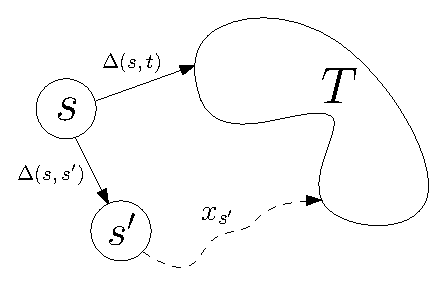
\includegraphics[scale=0.6]{figures/reachability.eps}
	%\caption{Illustration de l'accessibilité de l'état $s$ vers le sous-ensemble d'états $T$}
	\label{reachablity}
\end{figure}

\begin{itemize}
\renewcommand{\labelitemi}{\tiny$\bullet$}
	\item $ \sum_{s' \in S \setminus T}  \Delta(s, s') \cdot x_{s'} $ correspond à la probabilité que $s$ atteigne le sous-ensemble d'états $T$ en passant par un état intermédiaire $s' \in S \setminus T$.
	\item $\sum_{t \in T} \Delta(s, t)$ correspond à la probabilité que $s$ atteigne le sous-ensemble d'états $T$ en une seule étape.
\end{itemize}
Soit $n = |S|$. On obtient alors un système de $n$ équations à $n$ inconnues.

\begin{example}[\textit{Problème d'accessibilité}]\label{reachex}
	On considère la chaîne de Markov $\mathcal{M}_{re} = (S, \Delta)$ de la figure \ref{reachability-example} tel que $S = \{s_0, s_1, s_2, s_3, s_4, s_5, s_6\}$ et  $T = \{ s_5, s_6 \}$. On est intéressé par $\mathbb{P}_s(\Diamond T)$ pour tout $s \in S$.
	\begin{figure}[H]
	\centering
	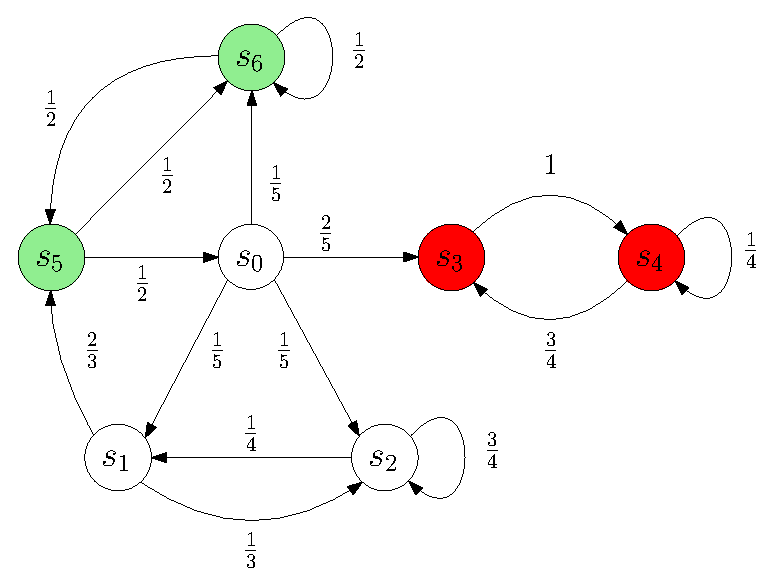
\includegraphics[scale=0.7]{figures/reachability-example.eps}
	\caption{Chaine de Markov sur laquelle on va résoudre le problème d'accessibilité.}
	\label{reachability-example}
	\end{figure}

Par le fait que $T = \{s_5, s_6\}$, on a que $x_{s_5} = x_{s_6} = 1$. Le graphe sous-jacent $G^{\mathcal{M}_{re}}$ permet de détecter que %la sous-chaîne absorbante composée des états $s_3$ et $s_4$ n'atteint jamais %
les états $s_3$ et $s_4$ ne sont pas connexes à $T$. Dès lors, on a que $x_{s_3} = x_{s_4} = 0$.
\[
\begin{cases}
x_{s_0} = \frac{1}{5} x_{s_1} + \frac{1}{5} x_{s_2} + \frac{2}{5} x_{s_3} + \frac{1}{5} \\
x_{s_1} = \frac{1}{3} x_{s_2} + \frac{2}{3} \\
x_{s_2} = \frac{1}{4} x_{s_1} + \frac{3}{4} x_{s_2} \\
x_{s_3} = 0 \\
x_{s_4} = 0 \\
x_{s_5} = 1 \\
x_{s_6} = 1
\end{cases}
\iff
\begin{cases}
x_{s_0} - \frac{1}{5} x_{s_1} - \frac{1}{5} x_{s_2} - \frac{2}{5} x_{s_3} = \frac{1}{5} \\
x_{s_1} - \frac{1}{3} x_{s_2} = \frac{2}{3} \\
\frac{-1}{4} x_{s_1} + \frac{1}{4} x_{s_2} = 0 \\
x_{s_3} = 0 \\
x_{s_4} = 0 \\
x_{s_5} = 1 \\
x_{s_6} = 1 
\end{cases}
\]

Afin de résoudre ce système, il est utile de le passer sous forme matricielle :

\[
\begin{pmatrix}
1 & \frac{-1}{5} & \frac{-1}{5} & \frac{-2}{5} & 0 & 0 & 0 \\[0.3em]
0 & 1 & \frac{-1}{3} & 0 & 0 & 0 & 0 \\[0.3em]
0 & \frac{-1}{4} & \frac{1}{4} & 0 & 0 & 0 & 0 \\[0.3em]
0 & 0 & 0 & 1 & 0 & 0 & 0 \\[0.3em]
0 & 0 & 0 & 0 & 1 & 0 & 0 \\[0.3em]
0 & 0 & 0 & 0 & 0 & 1 & 0 \\[0.3em]
0 & 0 & 0 & 0 & 0 & 0 & 1
\end{pmatrix}
\;
\begin{pmatrix}
x_{s_0} \\[0.3em] x _{s_1} \\[0.3em] x_{s_2} \\[0.3em] x_{s_3} \\[0.3em] x_{s_4} \\[0.3em] x_{s_5} \\[0.3em] x_{s_6}
\end{pmatrix}
= \;
\begin{pmatrix}
\; \frac{1}{5} \\[0.3em] \frac{2}{3} \\[0.3em] 0 \\[0.3em] 0 \\[0.3em] 0 \\[0.3em] 1 \\[0.3em] 1
\end{pmatrix}
\]

Ce système d'équations linéaires peut se résoudre par la méthode du \textit{pivot de Gauss}. %insérer ref cours d'anum de troest%
Dès lors, la solution de ce système est :
\[
x_{s_0} = \frac{3}{5}, \; x_{s_1} = 1, \; x_{s_2} = 1, \; x_{s_3} = 0, \; x_{s_4} = 0, \; x_{s_5} = 1, \; x_{s_6} = 1
\]
\end{example}


\begin{example}[\textit{Retour sur le dé de Knuth}]
	Reprenons la CM $\mathcal{M}_{Kd} = (S, \Delta)$ de l'exemple ~\ref{knuthdie}. Lorsqu'on lance un dé à $6$ faces, la probabilité d'obtenir n'importe quelle face de ce dé est de $\frac{1}{6}$. Dans $\mathcal{M}_{Kd}$, $s_0$ doit atteindre un des états finaux avec une probabilité $\frac{1}{6}$. On est donc intéressé de résoudre \[\mathbb{P}_{s_0}(\Diamond T) \text{ pour tout }T \in \{\{1\},\{2\},\{3\},\{4\},\{5\},\{6\}\} \]
	\`A l'aide du système défini dans cette sous-section, on calcule :
	\begin{spacing}{1.5}
	\begin{enumerate}
		\item $\mathbb{P}_{s_0} (\Diamond \{1\})$
		\begin{itemize}
			\renewcommand{\labelitemi}{\tiny$\bullet$}
			\item $x_1 = 1 $ car $1$ est l'état cible.
			\item $x_{s_{2, 3}} = x_{s_{4, 5, 6}} = x_{s_{4, 5}} = x_{s'_{4, 5, 6}} = x_2 = x_3 = x_4 = x_5 = x_6 = 0$ car ces sommets n'atteignent pas le sommet $1$ dans le graphe sous-jacent $G^{\mathcal{M}_{Kd}}$.
			\item $x_{s'_{1, 2, 3}} = \frac{1}{2} x_{s_{1, 2, 3}} + \frac{1}{2}$
			\item $x_{s_{1, 2, 3}} = \frac{1}{2} x_{s'_{1, 2, 3}} + \frac{1}{2}x_{s_{2, 3}} = \frac{1}{2} x_{s'_{1, 2, 3}} = \frac{1}{4} (x_{s_{1, 2, 3}} + 1) \Leftrightarrow
			4 x_{s_{1, 2, 3}} =x_{s_{1, 2, 3}} + 1 \Leftrightarrow x_{s_{1, 2, 3}} = \frac{1}{3}$
			%\item $x_{s'_{1, 2, 3}} = \frac{1}{6} + \frac{1}{2} = \frac{2}{3}$
			\item $x_{s_0} = \frac{1}{2} x_{s_{1,2,3}} + \frac{1}{2} x_{s_{4, 5, 6}} = \frac{1}{2} x_{s_{1,2,3}} = \frac{1}{6}$
		\end{itemize}
		\item $\mathbb{P}_{s_0} ( \Diamond \{2\})$
		\begin{itemize}
			\renewcommand{\labelitemi}{\tiny$\bullet$}
			\item $x_2 = 1 $ car $2$ est l'état cible.
			\item $x_{s_{4, 5, 6}} = x_{s_{4, 5}} = x_{s'_{4, 5, 6}} = x_1 = x_3 = x_4 = x_5 = x_6 = 0$ car ces sommets n'atteignent pas le sommet $2$ dans le graphe sous-jacent $G^{\mathcal{M}_{Kd}}$.
			\item $x_{s_{2, 3}} = \frac{1}{2} x_{s_3}  + \frac{1}{2} = \frac{1}{2} x_{s_2}$
			\item $x_{s'_{1, 2, 3}} = \frac{1}{2} x_{s_{1, 2, 3}} + \frac{1}{2} x_{s_1} = \frac{1}{2} x_{s_{1, 2, 3}}$
			\item $x_{s_{1, 2, 3}} = \frac{1}{2} x_{s'_{1, 2, 3}} + \frac{1}{2}  = 
			\frac{1}{2} (\frac{1}{2} x_{s_{1, 2, 3}}) +\frac{1}{2} (\frac{1}{2})
			= \frac{1}{4} x_{s_{1, 2, 3}} +\frac{1}{4}
			\Leftrightarrow \frac{3}{4} x_{s_{1, 2, 3}} = \frac{1}{4}
			\Leftrightarrow x_{s_{1, 2, 3}} = \frac{1}{3}$
			%\item $x_{s'_{1, 2, 3}} = \frac{1}{6} + \frac{1}{2} = \frac{2}{3}$
			\item $x_{s_0} = \frac{1}{2} x_{s_{1,2,3}} + \frac{1}{2} x_{s_{4, 5, 6}} = \frac{1}{2} x_{s_{1,2,3}} = \frac{1}{6}$
		\end{itemize}
		\item $\mathbb{P}_{s_0} (\Diamond \{3\}) = \frac{1}{6}$ (idem que $2.$).
	\end{enumerate}\end{spacing}
	Le comportement du système dans le cas où l'arc de droite est emprunté (\ie le résultat du premier lancer de pièce est pile) en $s_0$ est symétrique au cas où l'arc de gauche est emprunté (\cf exemple  ~\ref{knuthdie}). Dès lors, $\mathbb{P}_{s_0}(\Diamond \{4\}) = \mathbb{P}_{s_0}(\Diamond \{3\}) = \frac{1}{6}$ et $\mathbb{P}_{s_0}(\Diamond \{5\}) = \mathbb{P}_{s_0}(\Diamond \{2\}) = \frac{1}{6}$ et $\mathbb{P}_{s_0}(\Diamond \{6\}) = \mathbb{P}_{s_0}(\Diamond \{1\}) = \frac{1}{6}$. On a donc bien que le modèle simule un lancer de dé.
	
\end{example}

\subsection{Généralisation matricielle}
Le problème d'accessibilité pour la chaîne de Markov $\mathcal{M} = (S, \Delta)$ et le sous-ensemble d'états cibles $T \subseteq S$ peut résoudre par un système de $n$ équations à $n$ inconnues. On veut maintenant définir un système matriciel équivalent possédant une solution unique.\\

%Soit $\tilde{S}$, l'ensemble des états $s \in S \setminus T$ tel que il existe un chemin fini $\hat{\pi} \in Paths_{fin}^T(s)$. $\tilde{S}$ est donc l'ensemble des états de $S \setminus T$ connexes à $T$.
%Soient $\tilde{n} = |\tilde{S}|$, $i, j \in \{1 \dots n'\}$, et $s_i, s_j$ les $i^{\text{ème}} \text{ et } j^{\text{ème}} $ sommets de $\tilde{S}$. 
%\begin{itemize}
%\renewcommand{\labelitemi}{\tiny$\bullet$}
%\item Soit $A \in \mathbb{R}^{\tilde{n} \times \tilde{n}}$, la matrice de probabilité de transitions tel que $(Ax)_{i}$ indique la probabilité que $s_i$ atteigne $T$ via un état intermédiaire. Alors, $A_{i,j} = \Delta(s_i, s_j)$.
%\item Soit $b \in \mathbb{R}^{\tilde{n}}$ tel que $b_{i}$ est la probabilité que $s_i$ atteigne $T$ en une étape. Alors, $b_i = \sum_{t \in T} \Delta(s_i, t)$.
%\end{itemize}
%Le système matriciel correspondant est
%\[ x = Ax + b \]
%Cette équation peut être réécrite sous forme d'un système d'équations linéaires
%\[ (\mathbbm{1} - A) x = b \]
%avec $\mathbbm{1}$, la matrice unité de cardinalité $\tilde{n} \times \tilde{n}$ dans le but de le résoudre avec des algorithmes de résolution de systèmes d'équations linéaires (\eg $\;$avec le pivot de Gauss).\\
%La solution de ce système est \textbf{unique}

\begin{theorem}
	Soit $\mathcal{M} = (S, \Delta)$, une CM finie et $T \subseteq S$, un ensemble d'états cibles. On suppose que
	\begin{itemize}
		\renewcommand{\labelitemi}{\tiny$\bullet$}
		\item $S_{=0}$ est l'ensemble des états de $S$ non-connexes à $T$.
		\item $S_{=1} = T$.
		\item $S_? = S \setminus (S_{=1} \cup S_{=0})$
	\end{itemize}
	Alors, le vecteur $(\pr_s(\Diamond T))_{s \in S_?}$ est \textbf{l'unique solution} du système d'équations
	\[ x = Ax + b \]
	où 
	%Soient $n = |S|,\;  n^? = |S_?|, \; s_i$, le $i^\text{ème}$ somme de $S_?$ et $s_j$, le $j^\text{ème}$ sommet de $S_?$.
	\begin{itemize}
	\renewcommand{\labelitemi}{\tiny$\bullet$}
	\item $A \in \mathbb{Q}^{|S_?| \times |S_?|}$ est la matrice de probabilité de transitions telle que $\forall i, j \in \{1, \dots, |S_?| \}, \; A_{i, j} = \Delta(s_i, s_j)$. \\ $(Ax)_{i}$ correspond donc à la probabilité que $s_i$ atteigne $T$ via un état intermédiaire.
	\item $b \in \mathbb{Q}^{|S_?|}$ tel que $\forall i \in \{ 0, \dots, |S_?| \}, \; b_i = \sum_{t \in S_{=1}} \Delta(s_i, t)$. \\ $b_{i}$ correspond donc à la probabilité que $s_i$ atteigne $T$ en une étape. 
	\end{itemize}
\end{theorem}

%%% SOUS CHAINE ABSORBANTE ? %%%
%\subsection{Classe Finale}
%\begin{definition}[\textbf{\'Etat absorbant}]
%	Soit $\mathcal{M} = (S, \Delta)$, une CM. $s \in S$ est un \textit{état absorbant} de $\mathcal{M}$ \ssi $\Delta(s, s) = 1$.
%\end{definition}
%
%\begin{definition}[\textbf{Composante fortement connexe d'un graphe}]
%	Soit $G=(V, E)$, un graphe orienté dont $V$ est l'ensemble de sommets de $G$ et $E$ est l'ensemble des arcs de $G$. $B \subseteq V$ est une \textit{composante fortement connexe} de $G$ \ssi $\forall s,s' \in B,$ il existe un chemin $\pi = s_0 s_1 \dots s_n$ de $s$ à $s'$ tel que $s_0 = s , s_n = s'$ et $\forall i \in \{0 \dots n\}, s_i \in B$.
%\end{definition}
%
%\begin{definition}[\textbf{Classe finale}]
%	Soient $\mathcal{M} = (S, \Delta)$, une CM et $B \subseteq S$. Le sous-ensemble $B$ est une \textit{classe finale} de $\mathcal{M}$ \ssi $B$ est une composante fortement connexe de $G^\mathcal{M}$ et qu'aucun état en dehors de $B$ ne peut être atteint, \ie
%	\[\forall b \in B, \sum_{b' \in B} \Delta(b, b') = 1 \iff \sum_{s \in S \setminus B} \Delta(b, s) = 0\]
%\end{definition}
%
%\begin{propriete}
%		Soient $\mathcal{M}=(S, \Delta)$, une CM et $s \in S$ un état absorbant. L'ensemble $\{s\}$ est une classe finale de $\mathcal{M}$.
%\end{propriete}
%
%\begin{propriete}\label{BSCC-tip1}
%	Soient $\mathcal{M} = (S, \Delta)$, une CM et $T \subseteq S$, un ensemble d'états cibles. On suppose que les états de $B \subseteq S$ forment une classe finale de $\mathcal{M}$ et que $T \cap B = \emptyset$. Alors, $\forall b \in B, \; \mathbb{P}(b \models \Diamond T) = 0$.
%\end{propriete}
%
%\begin{propriete}[\textit{Application de la propriété ~\ref{BSCC-tip1}}]\label{Bscc-application} Soient $\mathcal{M} = (S, \Delta)$, une CM et $T \subseteq S$ un ensemble d'états cibles. On suppose que $B \subseteq S$ est une classe finale de $\mathcal{M}$ et que $T \cap B = \emptyset$. On construit la CM $\mathcal{M}' = (S', \Delta')$ où 
%\begin{itemize}
%\renewcommand{\labelitemi}{\tiny$\bullet$}
%\item $S' = \{s^*\} \cup S \setminus B$
%\item $s^*$ est un état absorbant
%\item $\forall s, s' \in S' \setminus \{s^*\}, \; \Delta'(s, s') = \Delta(s, s')$
%\item $ \forall s \in S', \Delta'(s, s^*) = \sum_{b \in B} \Delta(s, b)$
%\end{itemize}
%Alors, résoudre le problème d'accessibilité de $\mathcal{M}$ pour $T$ revient à résoudre le problème d'accessibilité de $\mathcal{M}'$ pour $T$. On dit que $\mathcal{M'}$ est induite par $B$.
%\end{propriete}
%	
%\begin{example}[\textit{Classe finale}]
%	Soient $\mathcal{M}_{re} = (S, \Delta)$, la CM de la figure \ref{reachability-example} et $T = \{s_5, s_6\}$, un ensemble d'états cibles. On a que les états $s_3$ et $s_4$ forment une classe finale de $\mathcal{M}_{re}$. La CM $\mathcal{M'}_{re}$ induite par cette classe finale est représentée à la figure ~\ref{absorbing-chain}
%		\begin{figure}[H]
%		\centering
%		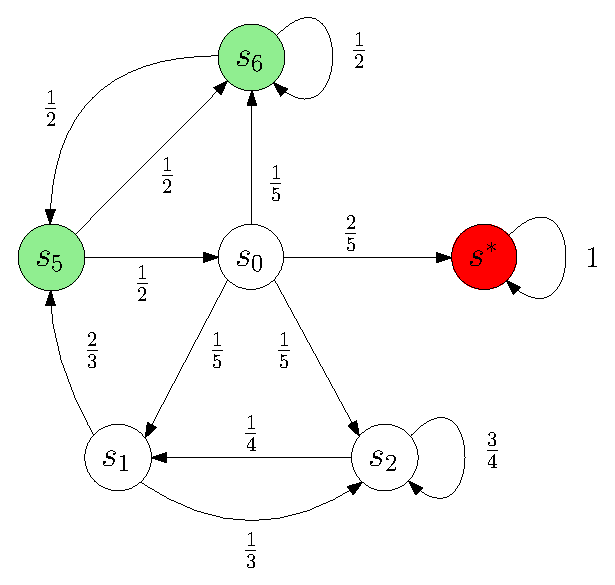
\includegraphics[scale=0.7]{figures/absorbing-chain.eps}
%		\caption{Chaine de Markov induite par la la classe finale formée par $s_3$ et $s_4$.}
%		\label{absorbing-chain}
%	\end{figure}
%\end{example}

\section{Plus court chemin dans une chaîne de Markov}
Il arrive qu'une chaîne de Markov classique ne soit pas suffisante pour modéliser un système, et plus particulièrement lorsque chaque transition a une répercussion différente sur un problème donné lié à ce système, \eg la quantité d'énergie utilisée pour passer d'un état à un autre dans un système à piles embarqué, la quantité d'argent dépensée lors d'une soirée au casino ou encore le temps écoulé pour atteindre une destination lors d'un voyage, $\dots$ \\
Les chaînes de Markov sont alors enrichies par une fonction de coût. Quitter un état pour en rejoindre un autre sera considéré comme une action pondérée, \ie chaque transition aura un coût en plus d'une probabilité. Dès lors, lorsqu'on s'intéresse aux chemins présents dans un tel automate et plus particulièrement à leur coût, un problème classique fait son apparition : quel sera le coût minimal pour atteindre un ensemble d'états cibles ? Les probabilités étiquetées sur les transitions de l'automate rendent le problème bien plus complexe qu'une recherche de plus court chemin dans un graphe pondéré. Dans cette section, deux approches seront étudiées. \textit{L'espérance du coût vers une cible} et \textit{l'accessibilité limitée par un coût}.

\begin{definition}[\textbf{Chaine de Markov pondérée}]
	Une \textit{chaîne de Markov pondérée}, notée \textbf{WCM}, est un tuple $\mathcal{M} = (S, \Delta, w)$ où
	\begin{itemize}
		\renewcommand{\labelitemi}{\tiny$\bullet$}
		\item $S$ et $\Delta$ sont définis comme pour une CM à temps discret.
		\item $w: S\times S \rightarrow \mathbb{Z}$ est la fonction de coût qui associe un poids entier sur chaque  transition, \ie pour toute transition $(s, s')$ telle que $s, s' \in S$ et $\Delta(s, s') > 0$.
	\end{itemize}
\end{definition}

\begin{remark}
	La représentation d'une WCM est la représentation de la CM correspondante où les poids sont ajoutés à côté des probabilités sur les étiquettes des transitions.
\end{remark}
\begin{example}[\textit{Production énergétique d'un système embarqué équipé de panneaux solaires}]\label{solar-pannel-example}
	Un système embarqué est alimenté par des panneaux solaires. Ceux-ci produisent chaque jour une certaine quantité d'énergie en fonction du climat : $5\; kJ$ les jours ensoleillés, $3\; kJ$ les jours légèrement nuageux, $2\; kJ$ les jours moyennement nuageux et $1\; kJ$ les jours fortement nuageux. Afin de modéliser ce système, on modélise d'abord la CM représentant les différents états du climat possibles chaque jour et on fixe ensuite la production énergétique sur les transition en tant que poids. La WCM correspondante est illustrée à la figure \ref{solar-pannel-1}
	
	\begin{figure}[H]
		\centering
		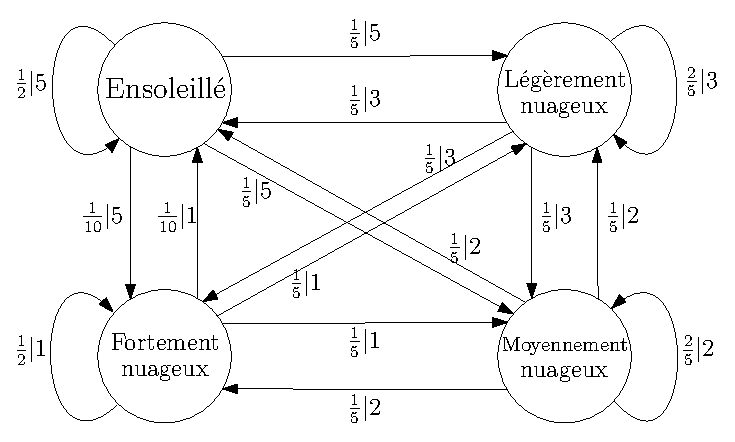
\includegraphics[scale=0.9]{figures/weather-solar-pannel.eps}
		\caption{Chaine de Markov pondérée de la production énergétique du système équipé de panneaux solaires en fonction du climat}
		\label{solar-pannel-1}
	\end{figure}
\end{example}

\begin{definition}[\textbf{Somme tronquée}]
	Soient $\mathcal{M} = (S, \Delta, w)$, une WCM, $T \subseteq S$, un sous-ensemble d'états cibles et $\pi = s_0s_1s_2 \dots \in Paths(\mathcal{M})$, un chemin dans $\mathcal{M}$. La \textit{somme tronquée} du chemin $\pi$ dans $\mathcal{M}$ pour $T$ est le coût total des transitions entre les états du chemin $\pi$ jusqu'à atteindre \textbf{pour la première fois} un des états cibles de $T$ (si le chemin n'atteint jamais un sommet de $T$, on dira que la somme tronquée est infinie).
	Plus strictement,
	soit $TS^T : Paths(\mathcal{M}) \rightarrow \mathbb{Z} \cup \infty$, la fonction qui calcule la somme tronquée de tout chemin vers l'ensemble cible $T$. La somme tronquée du chemin $\pi$ pour $T$ est définie par 
	\[
		TS^T(\pi) =
		\begin{cases}
			\sum_{i = 0}^{n-1} w(s_i, s_{i+1}) & \quad \text{si } \forall i \in \{0, \dots, n - 1\}, s_i \notin T \text{ et } s_n \in T \\
			+\infty & \quad \text{si } \pi \not \models \Diamond T,\; \ie \; \forall i \;\; s_i \notin T
		\end{cases}
	\]
\end{definition}

\begin{example}[\textit{Somme tronquée dans le système équipé de panneaux solaires}]
	Soit $\mathcal{M}_{sp}=(S, \Delta, w)$ la WCM de l'exemple \ref{solar-pannel-example}. On veut calculer l'énergie produite par les panneaux solaires cette semaine jusqu'à ce que le climat ait été fortement nuageux. On suppose que le temps était ensoleillé lundi, légèrement nuageux mardi et mercredi, ensoleillé jeudi, fortement nuageux vendredi et samedi ainsi que moyennement nuageux dimanche. Cette séquence forme un chemin $\pi = $\textit{ensoleillé, légèrement nuageux, légèrement nuageux, ensoleillé, fortement nuageux, fortement nuageux, moyennement nuageux} de $\mathcal{M}_{sp}$. Soit $T = \{\textit{fortement nuageux}\} \subseteq S$, l'ensemble cible. $TS^T(\pi) = 5 + 3 + 3 + 5 + 1 = 17$. Le système a donc produit $17\; kJ$ avant que le temps soit fortement nuageux. 
\end{example}

\begin{propriete}\label{prop-ts}
	Soient $\mathcal{M} = (S, \Delta, w)$, une WCM, $s \in S$, un état de $S$ et $T \subseteq S$, un ensemble d'états cibles. On suppose que $0 < \pr_s(\Diamond T) < 1$. Alors, cela signifie que $\exists s' \in S \text{ et } \exists \pi = s_0 \dots s_n \in Paths_{fin}(s)$ tel que $s_0 = s,\; s_n = s',\; s_i \notin T \text{ pour tout } i \in \{0, \dots n \} \text{ et } \forall \pi' \in Paths(s'), \; \pi' \not \models \Diamond T$, \ie \textit{il existe un chemin fini (qui ne passe pas par un état de $T$) dans $\mathcal{M}$ commençant en l'état $s$ et qui mène à un état $s'$ tel que $s'$ ne peut jamais atteindre $T$ via n'importe quel chemin dans $\mathcal{M}$.}\\ Dès lors, $TS^T(\pi') = \infty$ et donc $TS^T(\pi \cdot \pi') = \infty$, \ie \textit{tous les chemins commençant en $s$ dont $\pi$ est préfixe n'atteignent jamais $T$ et mènent à une somme tronquée infinie.}
\end{propriete}

\subsection{Problème de l'espérance du coût de l'accessibilité}
Dans cette section, on s'intéresse à l'espérance ~\ref{espmath} du coût des chemins qui atteignent un sous-ensemble d'états cibles d'une chaîne de Markov pondérée et plus précisément du coût total attendu pour qu'un état fixé atteigne un sous ensemble d'états cibles.

\begin{definition}[\textbf{Espérance du coût de l'accessibilité}]
	Soient $\mathcal{M} = (S, \Delta, w)$, une WCM, $s \in S$, un état de $s$ et $T \subseteq S$, un ensemble d'états cibles. kJ l'espérance $\mathbb{E}_s(TS^T)$, correspondant au \textit{coût total attendu pour atteindre $T$ depuis $s$} comme suit :
	\begin{itemize}
	\renewcommand{\labelitemi}{\tiny$\bullet$}
	\item 	Si $\pr_s(\Diamond T) < 1$, alors $\mathbb{E}_s(TS^T) = \infty$ (par la propriété \ref{prop-ts}).
	\item Sinon, \ie si $\pr_s(\Diamond T) = 1$, alors :
	\[ \mathbb{E}_s(TS^T) = \sum_{c = 0}^\infty c \cdot \pr_s(\{\pi \in Paths(s) \; | \; \pi \models \Diamond T \wedge TS^T(\pi) = c \})\]
	\end{itemize}
\end{definition}

\begin{proposition}
			Soit $Paths_{fin}^T(s)$, l'ensemble des chemins finis dans $\mathcal{M}$ commençant en $s$ de la forme $\hat{\pi} = s_0 \dots s_n$ où $s_0 = s, \;  s_i \notin T \; \text{ pour tout } i \in \{0, \dots, n-1\}$ et $s_n \in T$. Une définition équivalente de $\mathbb{E}_s(TS^T)$ dans le cas où $\pr_s(\Diamond T) = 1$ peut être donné par la moyenne du coût des chemins $\hat{\pi}$ pondérée par la probabilité de ces chemins $\hat{\pi}$ %alors que celui-ci se situe en l'état $s$
	, \ie
	\[\mathbb{E}_s(TS^T) = \sum_{\hat{\pi} \in Paths_{fin}^T(s)}\ \Delta(\hat{\pi}) \cdot TS^T(\hat{\pi})\]
\end{proposition}

\begin{proof}
	Soit $\pi = s_0 \dots s_n \dots \in Paths(s)$ tel que $\pi \models \Diamond T$. On suppose que $s_0 = s, \; \; s_i \notin T \; \text{ pour tout } i \in \{0, \dots, n-1\}$ et $s_n \in T$.  Soit $\hat{\pi} = s_0 \dots s_n \in Paths^T_{fin}(s)$. Alors, on a toujours que $TS^T(\pi) = TS^T(\hat{\pi})$.\\ \textit{(on peut ramener tout chemin infini $\pi$ qui atteint $T$ à un chemin fini $\hat{\pi}$ se terminant en la première occurrence d'un état de $T$ dans $\pi$ afin de calculer sa somme tronquée)}.
	\\Dès lors, soit $c \in \mathbb{N} \cup \infty,$
	\begin{flalign}
		& c \cdot \pr_s(\{\pi \in Paths(s) \; | \; \pi \models \Diamond T \wedge TS^T(\pi) = c \}) \notag\\
		& = c \cdot \pr_s(\{ \hat{\pi} \in Paths_{fin}^T(s) \; | \; TS^T(\hat{\pi}) = c\}) \notag\\
		& = c \cdot \sum_{\hat{\pi} \in Paths_{fin}^T(s) \; | \; TS^T(\hat{\pi}) = c} \Delta(\hat{\pi})
		\tag{car $\Delta$ induit la mesure $\pr_s$}\\
		& = \sum_{\hat{\pi} \in Paths_{fin}^T(s) \; | \; TS^T(\hat{\pi}) = c} \Delta(\hat{\pi}) \cdot c \notag \\
		& = \sum_{\hat{\pi} \in Paths_{fin}^T(s) \; | \; TS^T(\hat{\pi}) = c} \Delta(\hat{\pi}) \cdot TS^T(\hat{\pi})
		\tag{car $c = TS^T(\hat{\pi})$}\\
		&\iff \mathbb{E}_s(TS^T) = \sum_{c=0}^\infty \quad \sum_{\hat{\pi} \in Paths_{fin}^T(s) \; | \; TS^T(\hat{\pi}) = c} \Delta(\hat{\pi}) \cdot TS^T(\hat{\pi}) \notag\\
		&\iff \mathbb{E}_s(TS^T) = \sum_{\hat{\pi} \in Paths_{fin}^T(s)}\ \Delta(\hat{\pi}) \cdot TS^T(\hat{\pi}) \notag
	\end{flalign}
\end{proof}

\subsubsection*{Système d'équation linéaire}
Soient $\mathcal{M} = (S, \Delta, w)$, une WCM \textbf{finie}, $s\in S$, un état de $S$ et $T \subseteq$ S, un ensemble d'états cibles. Calculer $\mathbb{E}_s(TS^T)$ peut se calculer via un système d'équations linéaires comme suit : \\
%Soient $x_s = \mathbb{E}_s(TS^T)$ %et $S_{=1} = \{s \in S \; | \; \mathbb{P}_s_s(\Diamond T) = 1 \}$
Soit $succ(s)$, l'ensemble des successeurs de $s$ dans $G^\mathcal{M}$,
\[ x_s = 
	\begin{cases}
	\infty & \quad \text{si } \mathbb{P}_s(\Diamond T) < 1 \\
	0 & \quad \text{si } s \in T \\
	\sum_{s' \in succ(s)} \Delta(s, s') \cdot (w(s, s') + x_{s'}) & \quad \text{sinon}
	\end{cases}
\]

\begin{proposition}
	$x_s = \mathbb{E}_s(TS^T)$
\end{proposition}
\begin{proof}
	On prouve que $x_s = {E}_s(TS^T)$ par récurrence. \\
	\textbf{Cas de base :} 
	\begin{itemize}
	\renewcommand{\labelitemi}{\tiny$\bullet$}
		\item si $s \in T$, alors $x_s = 0$
		\item si $\pr_s(\Diamond T) = 0$ (on peut le vérifier à partir de $G^\mathcal{M}$), alors $x_s = \infty$
	\end{itemize}
	\textbf{Cas général :} Soit $n = |succ(s)|$. On suppose que $\forall i \in \{0, \dots, n-1 \}$ tel que $s_i \in succ(s), \; x_{s_i} = E_{s_i}(TS^T)$.\\
	Si $s \in T$ ou  $\pr_s(\Diamond T) = 0$, alors on est dans le cas de base. \\
	Si $\exists i \in \{0, \dots, n-1 \}$ tel que $\pr(s_i \models \Diamond T) < 1$, alors $x_{s_i} = \infty$ et \[x_s = \sum_{i \in \{0, \dots, n-1\}} \Delta(s, s_i) \cdot (w(s, s_i) + x_{s_i}) = \infty\]
	Sinon, alors $\forall i \in \{0, \dots, n-1 \},\; \pr(s_i \models \Diamond T) = 1$.\\
	Il reste à prouver que $x_s = \sum_{s \cdot \hat{\pi}} \Delta(s \cdot \hat{\pi})  \cdot TS^T(s \cdot \hat{\pi})$\\
	Soit $i \in \{0, \dots, n-1\}$. Supposons que $s_i \in T$. Alors,
	\begin{flalign}
		& \Delta(s, s_i) \cdot (w(s, s_i) + x_{s_i}) \notag \\
		& = \Delta(s, s_i) \cdot w(s, s_i)  \tag{car $x_{s_i} = 0$} \\
		& = \Delta(s, s_i) \cdot TS^T(s, s_i) \tag{a} \label{proof2-a}
	\end{flalign}
	Supposons à présent que $s_i \notin T$. Alors,
	$x_{s_i} = \sum_{\hat{\pi}} \Delta(\hat{\pi}) \cdot TS^T(\hat{\pi})$ et
	\begin{flalign}
		& \; \Delta(s, s_i) \cdot (w(s, s_i) + x_{s_i}) \notag \\
		= & \; \Delta(s, s_i) \cdot \Big(w(s, s_i) + \sum_{\hat{\pi} = s_i \dots t} \Delta(s_i \dots t) \cdot TS^T(s_i \dots t)\Big) \quad \text{$\forall t \in T$ tel que $\hat{\pi} \in Paths_{fin}^T$} \notag \\
		= & \; %\underbrace{
		\Delta(s, s_i) \cdot w(s, s_i)
		%}_{\text{espérance du coût de $s$ vers ses successeurs}}
		+ \sum_{\hat{\pi} = s_i \dots t} \Delta(s, s_i) \cdot \Delta(s_i \dots t) \cdot TS^T(s_i \dots t) \notag
	\end{flalign}
	\'Etant donné que $\pr(s_i \models \Diamond T) = 1$, que $s_i \notin T$ et que $\forall s, \sum_{s'} \Delta(s, s') = 1$, on a que 
	\begin{flalign}
		\sum_{\hat{\pi} = s_i \dots t} \Delta(\hat{\pi}) &= 1 \notag \\
		\iff \sum_{\hat{\pi} = s_i \dots t} \Delta(\hat{\pi}) \cdot w(s, s_i) &= w(s, s_i) \notag
	\end{flalign}
	Dès lors,
	\begin{flalign}
		& \;
		\Delta(s, s_i) \cdot w(s, s_i)
		+ \sum_{\hat{\pi} = s_i \dots t} \Delta(s, s_i) \cdot \Delta(s_i \dots t) \cdot TS^T(s_i \dots t)\notag \\
		= & \;
		\Delta(s, s_i) \cdot \Big(\sum_{\hat{\pi} = s_i \dots t} \Delta(s_i \dots t) \cdot w(s, s_i) \Big) + \Big(
		 \sum_{\hat{\pi} = s_i \dots t} \Delta(s, s_i) \cdot \Delta(s_i \dots t) \cdot TS^T(s_i \dots t) \Big)\notag \\
		 = & \;
		 \sum_{\hat{\pi} = s_i \dots t} \Delta(s, s_i) \cdot \Delta(s_i \dots t) \cdot w(s, s_i) + 
		 \sum_{\hat{\pi} = s_i \dots t} \Delta(s, s_i) \cdot \Delta(s_i \dots t) \cdot TS^T(s_i \dots t) \notag \\
		= & \sum_{\hat{\pi} = s_i \dots t} \Delta(ss_i \dots t) \cdot \Big(w(s, s_i) + TS^T(s_i \dots t) \Big) \notag \\
		= & \sum_{\hat{\pi} = s_i \dots t} \Delta(ss_i \dots t) \cdot TS^T(ss_i \dots t) \tag{b} \label{proof2-b}
	\end{flalign}
	Par \ref{proof2-a} et \ref{proof2-b}, on a :
	\begin{flalign}
		& \sum_{i \in \{0, \dots, n-1 \}} \Delta(s, s_i) (w(s, s_i) + x_{s_i}) \notag \\
		= & \quad \sum_{s \cdot \hat{\pi}} \Delta(s \cdot \hat{\pi}) \cdot TS^T(s \cdot \hat{\pi}) \notag
	\end{flalign}
\end{proof}

\begin{example}[\textit{Espérance de la production énergétique du système de panneaux solaires}]
	Cet exemple se base sur la WCM $\mathcal{M}_{sp} = (S, \Delta, w)$ de l'exemple \ref{solar-pannel-example}. On souhaite connaitre l'espérance de la production énergétique des panneaux solaires lorsque le climat est ensoleillé jusque quand le climat est fortement nuageux, dans le but de connaitre la production attendue que peut avoir une telle installation au moment où sa production est maximale jusqu'à son niveau de production minimale due au climat.\\
	Soit $s \in S$. On a $x_s = \mathbb{E}_s(TS^T)$. Le graphe $G^{\mathcal{M}_{sp}}$ est fortement connexe, on a donc $x_s \neq \infty$. Le système d'équations linéaires correspondant s'écrit :

\begin{flalign}
	&\begin{cases}
		x_{e} = \frac{1}{2} (5 + x_e) +
			\frac{1}{5} (5 + x_{ln}) +
			\frac{1}{5} (5 + x_{mn}) +
			\frac{1}{10} (5 + x_{fn}) \\
		x_{ln} = \frac{2}{5} (3 + x_{ln}) +
			\frac{1}{5} (3 + x_e) +
			\frac{1}{5} (3 + x_{mn}) +
			\frac{1}{5} (3 + x_{fn}) \\
		x_{ln} = \frac{2}{5} (2 + x_{mn}) +
			\frac{1}{5} (2 + x_e) +
			\frac{1}{5} (2 + x_{ln}) +
			\frac{1}{5} (2 + x_{fn}) \\
		x_{fn} = 0
	\end{cases}
	\notag\\
	\iff &\begin{cases}
		\frac{1}{2} x_e - \frac{1}{5} x_{ln} - \frac{1}{5} x_{mn} - \frac{1}{10}x_{fn} =5 \\
		\frac{-1}{5} x_e + \frac{3}{5} x_{ln} + \frac{1}{5} x_{mn} - \frac{1}{5} x_{fn} =3 \\
		\frac{-1}{5} x_e - \frac{1}{5} x_{ln} + \frac{3}{5} x_{mn} - \frac{1}{5} x_{fn} = 2 \\
		x_{fn} = 0
	\end{cases} \notag
\end{flalign}
Afin de résoudre ce système, il est utile de le passer sous forme matricielle :
\[
\begin{pmatrix}
\frac{1}{2} & \frac{-1}{5} & \frac{-1}{5} & \frac{-1}{10} \\[0.3em]
\frac{-1}{5} & \frac{3}{5} & \frac{-1}{5} & \frac{-1}{5} \\[0.3em]
\frac{-1}{5} & \frac{-1}{5} & \frac{3}{5} & \frac{-1}{5} \\[0.3em]
0 & 0 & 0 & 1
\end{pmatrix}
\;
\begin{pmatrix}
x_{e} \\[0.3em] x _{ln} \\[0.3em] x_{mn} \\[0.3em] x_{fn}
\end{pmatrix}
= \;
\begin{pmatrix}
\;5 \; \\[0.3em] \; 3 \; \\[0.3em] \; 2 \; \\[0.3em] \; 0 \;
\end{pmatrix}
\]
On résout encore une fois ce système d'équations linéaires par le pivot de Gauss. La solution du système est :
\[ x_e = 25, \; x_{ln} = 19.375, \; x_{mn} = 18.125, \; x_{fn} = 0  \]
De ce fait, $\mathbb{E}_{\textit{ensoleillé}} (TS^{\{\textit{fortement nuageux}\}}) = 25\; kJ$.
\end{example}

\subsection{Problème d'accessibilité limitée par un coût}
Dans le problème précédent, on était intéressé par le coût attendu pour qu'un état du système atteigne un sous-ensemble d'états cibles. Avec le \textit{problème d'accessibilité limitée par un coût}, on s'intéresse plutôt à la probabilité que cet état atteigne le sous-ensemble d'états cibles avec un coût inférieur à un seuil fixé au préalable.

\begin{definition}[\textbf{Accessibilité limitée par un coût}]
	Soient $\mathcal{M} = (S, \Delta, w)$, une WCM, $s \in S$, un état, $T \subseteq S$, un sous-ensemble d'états cibles et $b \in \mathbb{Z}$, un seuil. La \textit{probabilité d'atteindre $T$ depuis $s$ limitée par un coût} de seuil $b$ est définie comme suit : 
	\[\pr_s(TS^T \leq b) = \pr_s(\{\pi \in Paths(s) \; | \; TS^T(\pi) \leq b \}) \]
\end{definition}

\subsubsection*{Réduction au problème d'accessibilité}
Soient $\mathcal{M} = (S, \Delta, w)$, une WCM, $s \in S$, un état du système, $T \subseteq S$, un ensemble d'états cibles et $b \in \mathbb{Z}$, un seuil. Afin de résoudre $\pr_s(TS^T \leq b)$, on réduit le problème à un simple problème d'accessibilité sur la CM $\mathcal{M}' = (S', \Delta')$ pour le sous ensemble d'états cibles $T' \subseteq S'$. \\On construit $\mathcal{M'}$ comme suit :
\begin{itemize}
	\renewcommand{\labelitemi}{\tiny$\bullet$}
	\item $S'$ est un ensemble de tuples $(s, v)$ tel que $s \in S \cup \{s^*\}$ et $v \in \mathbb{Z} \cup \{ \bot \}$. On considère que $\bot > b$. Intuitivement, on enregistre dans $v$ le coût total du chemin en parcourant $\mathcal{M}$. Les états cibles sont donc les états de $T' = \{ (s, v) \in S' \; | \; s \in T \wedge v \leq b \}$.
	\item $\Delta^*: S' \times S' \rightarrow [0,1]$ est la fonction de probabilité de transition intermédiaire, définie comme suit :\\
	$\forall (s, v), (s', v') \in S',$
	\[
		\Delta^*((s, v), (s', v')) = 
		\begin{cases}
		\Delta(s, s') & \text{\quad \, si $v' = v + w(s, s')$ et $v' \leq b$  et $s \notin T$ } \\
		 & \text{ou si $v' = \bot$ et $v + w(s, s') > b$  et $s \notin T$} \\
		 1 & \quad \, \text{ si $s = s' \in T$ et $v = v'$} \\
		 0 & \quad \, \text{ sinon}
		\end{cases}
	\]

\begin{remark}
	Nous ne sommes intéressés que par les chemins dont le coût total (\ie la somme tronquée) est inférieur à $b$. De ce fait, tout état $(s, v) \in S'$ tel que $v = \bot$ n'est utile au système que pour identifier les chemins qui ont dépassé le seuil $b$. Soient $\mathcal{M^*}$, une CM qu'on a construit à partir de $\mathcal{M}$ telle que $\mathcal{M^*} = (S', \Delta^*)$ et $S^* \subseteq S'$, l'ensemble des états $(s, v) \in S'$ tel que $v = \bot$. Par le fait que $T' \cap S^* = \emptyset$ ainsi que par le fait que $\forall (s, v) \in S^*$, tout chemin $\pi$ de $\mathcal{M^*}$ tel que $\pi \in Paths((s, v))$ vérifie $\pi \not \models \Diamond T'$, on peut remplacer tout état de $S^*$ dans $\mathcal{M^*}$ par un seul état absorbant $(s^*, \bot)$ dans $\mathcal{M'}$ . \\
\end{remark}

\item $\Delta': S' \times S' \rightarrow [0,1]$ est la fonction de probabilité de transition de $\mathcal{M'}$ et est définie comme suit : \\
	$\forall (s, v), (s', v') \in S',$
\[
\Delta'((s, v), (s', v')) =  
\begin{cases}
\Delta(s, s') & \text{\quad \, si $v' = v + w(s, s')$ et $v' \leq b$}  \\
	& %\quad \quad \;\,
	\quad \;\, \text{et $s \notin T$} \\
\sum_{(s_\bot, v_\bot) \in S' | v_\bot = \bot} \Delta^*((s, v), (s_\bot, v_\bot)) & \quad \, \text{ si $s' = s^*$ et $v' = \bot$} \\
1 & \quad \, \text{ si $s = s' \in T$ et $v = v'$} \\
& \text{ou si $s = s' = s^*$ et $v = v' = \bot$} \\
0 & \quad \, \text{ sinon}
\end{cases}
\]
\end{itemize}
 Dès lors, on a \[\pr^\mathcal{M}_s(\{\pi \in Paths(s) \; | \; TS^T(\pi) \leq b \}) = \pr^\mathcal{M'}((s, 0) \models \Diamond T')\]
\ie résoudre le problème d'accessibilité de $s$ à $T$ dans $\mathcal{M}$ limitée par le coût de seuil $b$ revient à résoudre le problème d'accessibilité de $(s, 0)$ à $T'$ dans $\mathcal{M'}$.

\begin{example}[\textit{Accessibilité limitée par un coût dans le système équipé de panneaux solaires}]
	On reprend la WCM $\mathcal{M}_{sp} = (S, \Delta, w)$ de l'exemple \ref{solar-pannel-example}. 
	%On suppose que l'installation de panneaux solaire est rentable lorsque celle-ci produit au moins $8\; kJ$ lorsque le climat est ensoleillé jusque quand le climat est fortement nuageux.
	On souhaite connaitre la probabilité que le système équipé de panneaux solaires produise \textbf{au moins $8 \; kJ$} avant que le climat soit fortement nuageux, en supposant que l'installation commence à produire l'énergie un jour ensoleillé.\\
	Pour ce faire, on va d'abord déterminer la probabilité que le système produise moins de $7\; kJ$, \ie $\pr_{\textit{ensoleillé}}(TS^{\{ \textit{fortement nuageux} \}} \leq 7)$. On réduit le problème à un problème d'accessibilité en construisant la CM $\mathcal{M'}_{sp} = (S', \Delta')$ comme décrit ci-dessus (\cf figure \ref{figure-cbr-03}).
	
\begin{figure}[H]
	\centering
	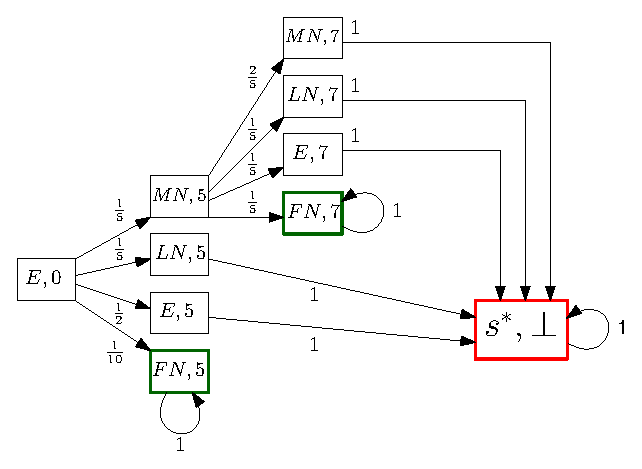
\includegraphics[scale=1]{figures/cost-bounded-reachability03.eps}
	\caption{CM $\mathcal{M'}_{sp}$ construite à partir de $\mathcal{M}_{sp}$ afin de résoudre $\pr_{\textit{ensoleillé}}(TS^{\{ \textit{fortement nuageux} \}} \leq 7)$}
	\label{figure-cbr-03}
\end{figure}
Dès lors, $T' = \{ (FN, 5), (FN, 7) \}$. Il reste à résoudre le problème d'accessibilité $\pr((E, 0) \models \Diamond T')$ : 
\begin{flalign}
	&x_{(LN, 5)} = x_{(E, 5)} = x_{(MN, 7)} = x_{(E, 7)} = x_{(s^*, \bot)} = 0 \notag \\ 
	&\begin{cases}
		x_{(E, 0)} = \frac{1}{5} x_{(MN, 5)} + \frac{1}{5} x_{(LN, 5)} + \frac{1}{2} x_{(E, 5)} + \frac{1}{10} \\
		x_{(MN, 5)} = \frac{2}{5} x_{(MN, 7)} + \frac{1}{5} x_{(LN, 7)} + \frac{1}{5} x_{(E, 7)} + \frac{1}{5}
	\end{cases}\notag \\
	\iff &
	\begin{cases}
		x_{(E, 0)} = \frac{1}{5} x_{(MN, 5)} + \frac{1}{10} \\
		x_{(MN, 5)} = \frac{1}{5}
	\end{cases}\notag \\
	\implies& x_{(E, 0)} = \frac{7}{50} = 0.14 \notag
\end{flalign}
On a $\pr^{\mathcal{M'}}((E, 0) \models \Diamond T') = \pr^\mathcal{M}_{\textit{ensoleillé}}(TS^{\{ \textit{fortement nuageux} \}} \leq 7) = 0.14$. On revient au problème initial. On veut connaitre $\pr_{\textit{ensoleillé}}(TS^{\{ \textit{fortement nuageux} \}} > 7)$. Comme $\pr_{\textit{ensoleillé}}$ est une mesure de probabilité, on a \[1 - \pr_{\textit{ensoleillé}}(TS^{\{ \textit{fortement nuageux} \}} \leq 7) = \pr_{\textit{ensoleillé}}(TS^{\{ \textit{fortement nuageux} \}} > 7)\]
Et donc, on a $\pr_{\textit{ensoleillé}}(TS^{\{ \textit{fortement nuageux} \}} > 7) = 0.86$.
\end{example}
%\begin{example}[\textit{Réduction au problème d'accessibilité}]
%	Pour cet exemple, reprenons la CM de l'exemple \ref{reachex} en ajoutant des poids sur les transitions. On obtient la WCM $\mathcal{M}_{cbr}$ (\cf figure \ref{figure-cbr-01}).
%	
%	\begin{figure}[H]
%		\centering
%		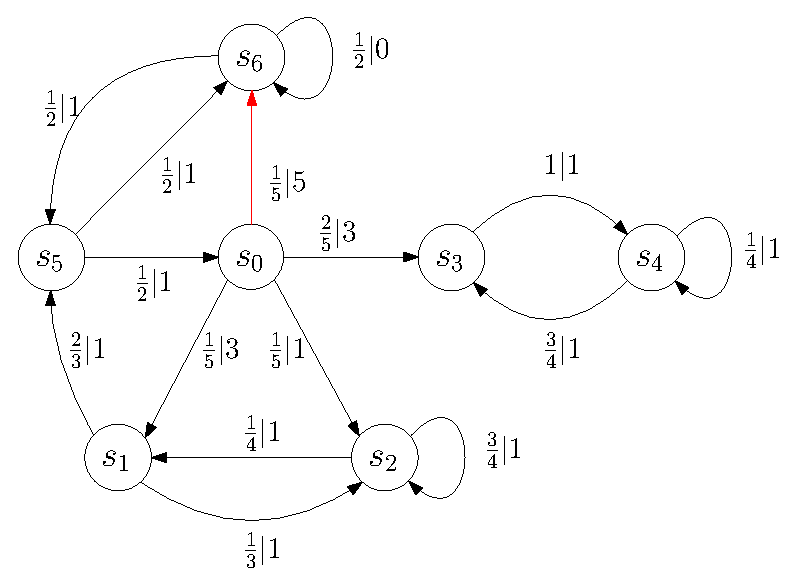
\includegraphics[scale=0.7]{figures/cost-bounded-reachability01.eps}
%		\caption{Chaine de Markov pondérée $\mathcal{M}_{cbr}$}
%		\label{figure-cbr-01}
%	\end{figure}
%
%	On souhaite connaitre la probabilité que le fait de ne pas emprunter la transition $(s_0, s_6)$ soit avantageux au niveau du coût total pour atteindre les états $s_5$ ou $s_6$ depuis $s_0$, ou encore la probabilité d'atteindre les états $s_5$ ou $s_6$ depuis l'état $s_0$ avec un coût strictement inférieur à $5$ \ie $\pr_{s_0}(\{ \pi \in Paths(s_0) \; | \; TS^T(\pi) \leq 4 \})$. Pour cela, on réduit le problème à un problème d'accessibilité sur la WCM $\mathcal{M}'_{cbr}$ (\cf figure \ref{figure-cbr-02}). Dès lors, l'ensemble d'états cibles est $T' = \{ (s_5, 4), (s_5, 3), (s_6, 4) \}$.
%	
%	\begin{figure}[H]
%		\centering
%		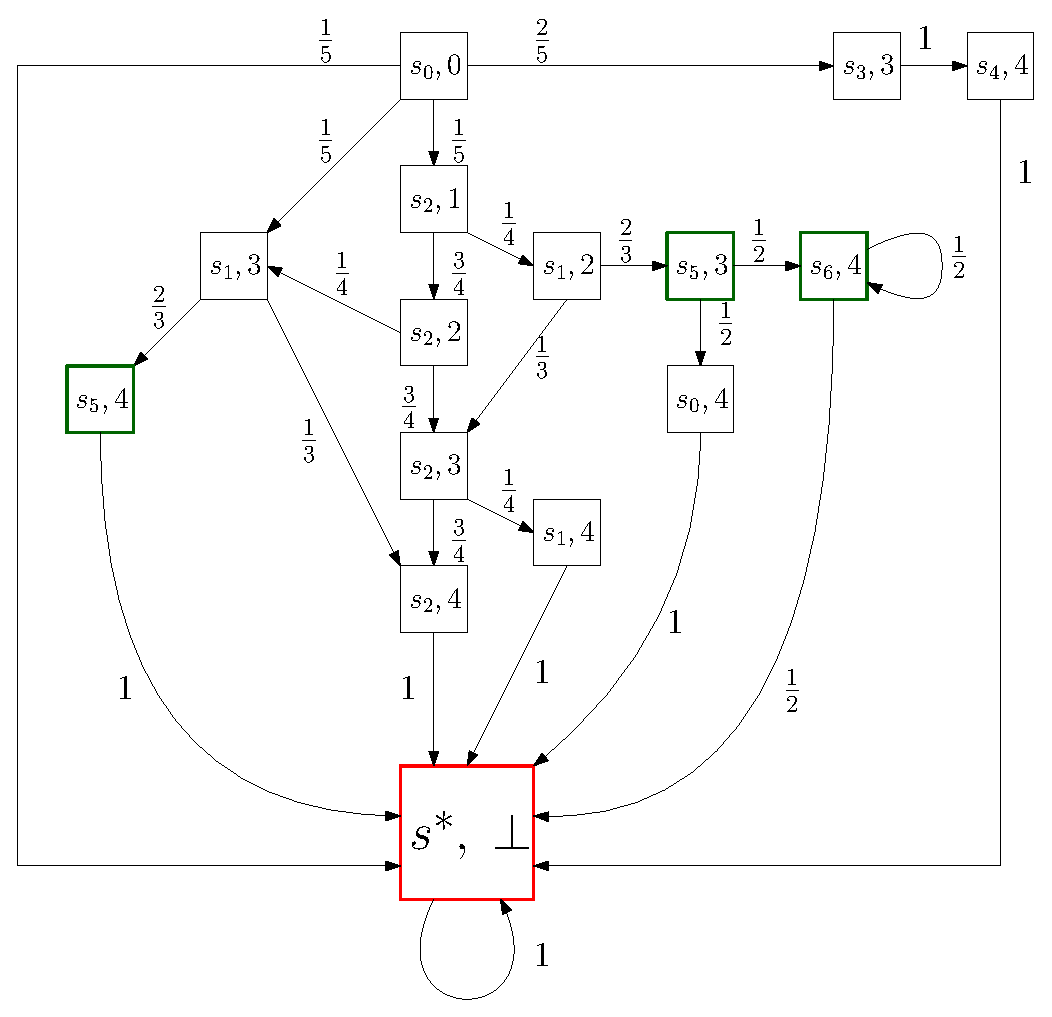
\includegraphics[scale=0.5]{figures/cost-bounded-reachability02.eps}
%		\caption{WCM $\mathcal{M'}_{cbr}$ construite à partir de $\mathcal{M}_{cbr}$ dans le but de résoudre le problème $\pr_{s_0}(\{ \pi \in Paths(s_0) \; | \; TS^T(\pi) \leq 4 \})$ }
%		\label{figure-cbr-02}
%	\end{figure}
%\end{example}
\bibliography{bib}{}
\bibliographystyle{plain}

\end{document}